%% MODELO DE LATEX PARA TRABALHOS ACADÊMICOS
%% INSTRUÇÕES GERAIS:
%%    1. TODO O TEXTO NA FRENTE DO SIMBOLO '%' É COMENTÁRIO, ISTO É, ELE NÃO FAZ DIFERENÇA NO RESULTADO FINAL 
%%    2. NESTE MODELO, VOCÊS SÓ PRECISAM EDITAR DAS LINHAS 114 A 132 (INFORMAÇÕES DE CAPA) E DAS LINHAS 188 EM DIANTE (CORPO DO TRABALHO). O RESTO SÃO CONFIGURAÇÕES DE FORMATAÇÃO QUE PROVAVELMENTE NÃO SERÁ PRECISO MODIFICAR.
%%    3. MAIS INSTRUÇÕES DETALHADAS PODERÃO SER ENCONTRADAS NA PÁGINA profhelioh.wordpress.com. DÚVIDAS: heliohenrique@ufpr.br OU heliohenrique3@gmail.com

% INFORMAÇÕES DA FONTE:
%% abtex2-modelo-relatorio-tecnico.tex, v-1.7.1 laurocesar
%% Copyright 2012-2013 by abnTeX2 group at http://abntex2.googlecode.com/ 
%%
%% This work may be distributed and/or modified under the
%% conditions of the LaTeX Project Public License, either version 1.3
%% of this license or (at your option) any later version.
%% The latest version of this license is in
%%   http://www.latex-project.org/lppl.txt
%% and version 1.3 or later is part of all distributions of LaTeX
%% version 2005/12/01 or later.
%%
%% This work has the LPPL maintenance status `maintained'.
%% 
%% The Current Maintainer of this work is the abnTeX2 team, led
%% by Lauro César Araujo. Further information are available on 
%% http://abntex2.googlecode.com/
%%
%% This work consists of the files abntex2-modelo-relatorio-tecnico.tex,
%% abntex2-modelo-include-comandos and abntex2-modelo-references.bib
%%
% ------------------------------------------------------------------------
% ------------------------------------------------------------------------
% abnTeX2: Modelo de Relatório Técnico/Acadêmico em conformidade com 
% ABNT NBR 10719:2011 Informação e documentação - Relatório técnico e/ou
% científico - Apresentação
% ------------------------------------------------------------------------ 
% ------------------------------------------------------------------------

\documentclass[
	% -- opções da classe memoir --
	12pt,				% tamanho da fonte
	% openright,			% capítulos começam em pág ímpar (insere página vazia caso preciso)
    oneside,			% para impressão somente frente. Oposto a twoside (frente e verso)
	a4paper,			% tamanho do papel. 
	% -- opções da classe abntex2 --
	%chapter=TITLE,		% títulos de capítulos convertidos em letras maiúsculas
	%section=TITLE,		% títulos de seções convertidos em letras maiúsculas
	%subsection=TITLE,	% títulos de subseções convertidos em letras maiúsculas
	%subsubsection=TITLE,% títulos de subsubseções convertidos em letras maiúsculas
	% -- opções do pacote babel --
	english,			% idioma adicional para hifenização
	french,				% idioma adicional para hifenização
	spanish,			% idioma adicional para hifenização
	brazil,				% o último idioma é o principal do documento
	]{abntex2}


% ---
% PACOTES
% ---

% ---
% Pacotes fundamentais 
% ---
\usepackage{cmap}				% Mapear caracteres especiais no PDF
\usepackage{lmodern}			% Usa a fonte Latin Modern
\usepackage[T1]{fontenc}		% Selecao de codigos de fonte.
\usepackage[utf8]{inputenc}		% Codificacao do documento (conversão automática dos acentos)
\usepackage{indentfirst}		% Indenta o primeiro parágrafo de cada seção.
\usepackage{color}				% Controle das cores
\usepackage{graphicx}			% Inclusão de gráficos
% ---

% ---
% Pacotes adicionais, usados no anexo do modelo de folha de identificação
% ---
\usepackage{multicol}
\usepackage{multirow}
% ---
	
% ---
% Pacotes adicionais, usados apenas no âmbito do Modelo Canônico do abnteX2
% ---
\usepackage{lipsum}				% para geração de dummy text
% ---

% ---
% Pacotes de citações
% ---
\usepackage[brazilian,hyperpageref]{backref}	 % Paginas com as citações na bibl
\usepackage[alf]{abntex2cite}	% Citações padrão ABNT

% --- 
% CONFIGURAÇÕES DE PACOTES
% --- 

% ---
% Configurações do pacote backref
% Usado sem a opção hyperpageref de backref
\renewcommand{\backrefpagesname}{Citado na(s) página(s):~}
% Texto padrão antes do número das páginas
\renewcommand{\backref}{}
% Define os textos da citação
\renewcommand*{\backrefalt}[4]{
	\ifcase #1 %
		Nenhuma citação no texto.%
	\or
		Citado na página #2.%
	\else
		Citado #1 vezes nas páginas #2.%
	\fi}%
% ---

% ---
% Informações de dados para CAPA e FOLHA DE ROSTO
% ---
\titulo{Trabalho de Informática}
\autor{Fulano da Silva}
\local{Brasil}
\data{20 de novembro de 2014}
\instituicao{%
  Universidade Federal do Paraná
  \par
  Setor Palotina
  \par
  Engenharia de Aquicultura}
\tipotrabalho{Relatório técnico}
% O preambulo deve conter o tipo do trabalho, o objetivo, 
% o nome da instituição e a área de concentração 
\preambulo{Modelo canônico de Relatório Técnico e/ou Científico em conformidade
com as normas ABNT apresentado à comunidade de usuários \LaTeX.}
% ---

% ---
% Configurações de aparência do PDF final

% alterando o aspecto da cor azul
\definecolor{blue}{RGB}{41,5,195}

% informações do PDF
\makeatletter
\hypersetup{
     	%pagebackref=true,
		pdftitle={\@title}, 
		pdfauthor={\@author},
    	pdfsubject={\imprimirpreambulo},
	    pdfcreator={LaTeX with abnTeX2},
		pdfkeywords={abnt}{latex}{abntex}{abntex2}{relatório técnico}, 
		colorlinks=true,       		% false: boxed links; true: colored links
    	linkcolor=blue,          	% color of internal links
    	citecolor=blue,        		% color of links to bibliography
    	filecolor=magenta,      		% color of file links
		urlcolor=blue,
		bookmarksdepth=4
}
\makeatother
% --- 

% --- 
% Espaçamentos entre linhas e parágrafos 
% --- 

% O tamanho do parágrafo é dado por:
\setlength{\parindent}{1.3cm}

% Controle do espaçamento entre um parágrafo e outro:
\setlength{\parskip}{0.2cm}  % tente também \onelineskip

% ---
% compila o indice
% ---
\makeindex
% ---

% ----
% Início do documento
% ----
\begin{document}

% Retira espaço extra obsoleto entre as frases.
\frenchspacing 

% ----------------------------------------------------------
% ELEMENTOS PRÉ-TEXTUAIS
% ----------------------------------------------------------
% \pretextual

% ---
% Capa
% ---
\imprimircapa
% ---

% ---
% Folha de rosto
% (o * indica que haverá a ficha bibliográfica)
% ---
\imprimirfolhaderosto*
% ---


% ---
% Agradecimentos
% ---
\begin{agradecimentos}
O agradecimento principal é direcionado a Youssef Cherem, autor do
\nameref{formulado-identificacao} (\autopageref{formulado-identificacao}).

Os agradecimentos especiais são direcionados ao Centro de Pesquisa em
Arquitetura da Informação\footnote{\url{http://www.cpai.unb.br/}} da Universidade de
Brasília (CPAI), ao grupo de usuários
\emph{latex-br}\footnote{\url{http://groups.google.com/group/latex-br}} e aos
novos voluntários do grupo
\emph{\abnTeX}\footnote{\url{http://groups.google.com/group/abntex2} e
\url{http://abntex2.googlecode.com/}}~que contribuíram e que ainda
contribuirão para a evolução do abn\TeX.

\end{agradecimentos}
% ---

% ---
% RESUMO
% ---

% resumo na língua vernácula (obrigatório)
\begin{resumo} %% AQUI COMEÇA A PÁGINA DE RESUMO
 Segundo a \citeonline{NBR6028:2003}, o resumo deve ressaltar o
 objetivo, o método, os resultados e as conclusões do documento. A ordem e a extensão
 destes itens dependem do tipo de resumo (informativo ou indicativo) e do
 tratamento que cada item recebe no documento original. O resumo deve ser
 precedido da referência do documento, com exceção do resumo inserido no
 próprio documento. (\ldots) As palavras-chave devem figurar logo abaixo do
 resumo, antecedidas da expressão Palavras-chave:, separadas entre si por
 ponto e finalizadas também por ponto. Bla bla bla bla bla \cite{fulano} %% EXEMPLO DE CITAÇÃO (vá em abntex2-modelo-references.bib)

 \vspace{\onelineskip}
    
 \noindent
 \textbf{Palavras-chaves}: latex. abntex. editoração de texto.
\end{resumo} %AQUI TERMINA A PÁGINA DE RESUMO
% ---

% ---
% inserir lista de ilustrações
% ---

\listoffigures* %% o * indica que não será incluso no sumário
\cleardoublepage %% Pula página
% ---

% ---
% inserir lista de tabelas
% ---

\listoftables*
\cleardoublepage
% ---

% ---
% inserir lista de abreviaturas e siglas
% ---
\begin{siglas}
  \item[Fig.] Area of the $i^{th}$ component
  \item[456] Isto é um número
  \item[123] Isto é outro número
  \item[lauro cesar] este é o meu nome
\end{siglas}
% ---

% ---
% inserir lista de símbolos
% ---
\begin{simbolos}
  \item[$ \Gamma $] Letra grega Gama
  \item[$ \Lambda $] Lambda
  \item[$ \zeta $] Letra grega minúscula zeta
  \item[$ \in $] Pertence
\end{simbolos}
% ---

% ---
% inserir o sumario
% ---

\tableofcontents*

% ---

% ----------------------------------------------------------
% ELEMENTOS TEXTUAIS  (necessário para incluir número nas páginas)
% ----------------------------------------------------------
\textual


% ----------------------------------------------------------
% Introdução
% ----------------------------------------------------------
\chapter{Introdução}\label{Introdução}

Neste capítulo é apresentada a motivação do presente estudo, assim como seus objetivos e sua organização.

\section{Motivação}

O comportamento do motorista afeta em grande parte a segurança no transito \cite{evans2004traffic}, estima-se que 856,000 acidentes de estrada ocorrem anualmente, sendo 74\% deles em países subdesenvolvidos (\citeauthor{worldhealthorganization2018}, \citeyear{worldhealthorganization2018}). Em 2004, os acidentes de trânsito representavam a nona mais importante causa de morte no mundo, com 1,2 milhão de vítimas \cite{bacchieri2011acidentes} A OMS estima que em 2030 subirão para a quinta posição. Felizmente, estudos mostram que é possível adaptar o comportamento do condutor de forma a aumentar a segurança, diminuir o consumo de combustível e as emissões de gases dos veículos \cite{goldberg2000} \cite{almazan2013full}. Em vista disso, a Análise de Perfil de Motorista (APM) se apresenta como uma forma de melhorar o comportamento do motorista, levando ele a uma condução mais segura e consciente. (\citeauthor*{zheng2016unsupervised}, \citeyear{zheng2016unsupervised}; \citeauthor{castignani2015driver},  \citeyear{castignani2015driver})

A APM consiste na coleta de dados de condução através de diversos sensores e em seguida a aplicação de um modelo computacional a fim de gerar pontos ou uma classificação que caracterize a forma de dirigir do motorista (\citeauthor*{eren2012estimating}, \citeyear{eren2012estimating}). Nesse sentido são apresentados diversos estudos que analisam hábitos de direção. Grande parte deles utilizam uma vasta gama de sensores do próprio veículo, tal como sensores externos (câmeras, microfones e radares). 
smartfones modernos oferecem sensores adequados para coletar dados para a análise de perfil de condutor \cite{junior2017driver}. Trabalhos anteriores (**citar trabalhos**) demonstram a alta correlação entre as medições de sensores embarcados em dispositivos smartfones e caixas telemáticas instaladas fixamente nos veículos. Embora haja espaço para desenvolvimento e melhorias, os smartfones se provaram uma forma conveniente de se instrumentar a coleta de dados em um veículo.

Em linhas gerais a APM tem se tornado cada vez mais relevante. \citeauthor{junior2017driver} \cite{junior2017driver} destaca que telemática de seguros, particularmente, tem se apropriado da tecnologia de forma a  tornar mais barato o valor da franquia para motoristas com boas pontuações, ao invés de usar apenas estatísticas que dizem respeito a grupos (e.g, idade, sexo, estado civil).

É observada na literatura diversos trabalhos (\cite{Paefgen:2012:DBA:2406367.2406412},\cite{eren2012estimating}) que utilizam alguma especie de fusão de sensores para classificar a corrida de motoristas. \citeauthor{araujo2012driving} criou um Aplicativo com o objetivo de conscientizar os motoristas no que diz respeito ao consumo de combustível. Para tal, se utilizam os sensores do smartfone(GPS) e o estado do veículo(velocidade, combustível, aceleração, etc.), processados através de um algoritmo que utiliza lógica fuzzy. Em seguida o consumo é comparado com com métricas providas pela montadora do carro. Os resultados preliminares mostram um potencial de redução do consumo de combustível e a mudança no comportamento do motorista.

Outro trabalho \citep{chen2015d} propõem a identificar movimentos de direção agressivos, através da análise dos sensores de GPS e acelerômetro de um dispositivo smartfone. A princípio, os eixos do carro e do aparelho são alinhados manualmente, fazendo sentido dos dados observados pela captura de sensores. Para detecção de eventos, o algoritmo compara o desvio padrão da assinatura e a média, com alguns limiares, de forma a observar o início de um evento. Depois de iniciado o algoritmo monitora as médias e os desvios padrões nos eixos para constatar que o evento chegou ao fim. Em seguida a janela armazenada alimenta uma SVM que é capaz de detectar e distinguir com 95.36\% de acurácia 6 eventos de direção.

\begin{figure}
    \centering
    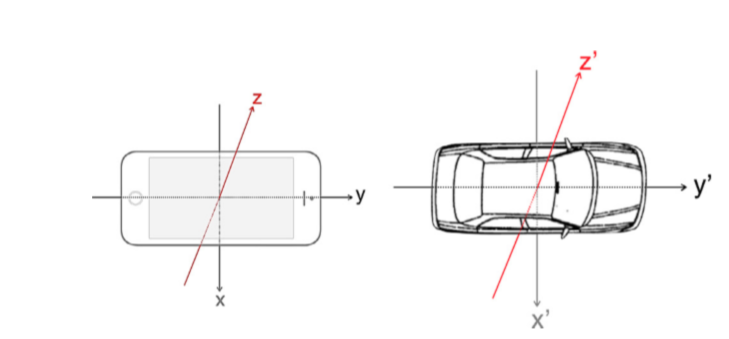
\includegraphics[width = 150mm]{Figuras/celularcarro.PNG}
    \caption{Sistema de Coordenadas do Celular Alinhado com Sistema de Coordenadas do Veículo\\Fonte: \citeauthor{vlahogianni2017driving} (\citeyear{vlahogianni2017driving})}
    \label{fig:celularCarroAlinhados}
\end{figure}{}


No entanto, em um caso prático, dificilmente o dispositivo móvel se encontra com o eixo dos seus sensores alinhados com o carro (conforme exemplificado pela Figura \ref{fig:celularCarroAlinhados}). Nesse caso, empobrece-se a analise e quantidade de informação que se pode extrair de uma viagem, no que tange ao comportamento do motorista. Diversos trabalhos que buscam realizar a APM através dos dados coletados através de dispositivos smartfones, recorrem ao alinhamento manual do aparelho com o carro ou a transformação de eixos para o sistema de coordenadas global. O primeiro método possui como limitante, a variabilidade da posição do dispositivo em um caso real de uso.

O segundo método deve lançar mão do magnetômetro embarcado no dispositivo. Esse sensor aparece cada vez mais nos dispositivos ao longo dos anos, porém de acordo com a Tabela \ref{tab:aparelhosMaisVendidos}, 50\% dos aparelhos mais vendidos em 2018 não possuíam o magnetômetro, o que pode se tornar um gargalo para adoção ampla do método. Em suma, o magnetômetro funciona como uma espécie de bussola, devido a capacidade do sensor de captar tanto campos magnéticos locais como o campo magnético terrestre. Nesse sentido, o sensor é utilizado em conjunto com o sensor de gravidade - um sensor virtual, que é obtido através de uma filtragem de baixa no acelerômetro -, com o objetivo de migrar o sistema de coordenadas local do celular, para um sistema de coordenadas global. No entanto, é mostrado na literatura(**citar**) que a sensibilidade do magnetômetro é alta, e suas medições são alteradas na presença de pequenos campos magnéticos e objetos metálicos. Uma vez que a gama de eletro-eletrônicos embarcados em um veículo só tende a aumentar, devido a maior interconectividade entre os sistemas do carro, a medição do campo captado por esse sensor se torna cada vez mais imprecisa. Outro aspecto dessa problemática advém de que um sistema de coordenadas global diz pouco a respeito da dinâmica veicular observada no carro.


\begin{table}[]
\centering
\caption{Presença do Magnetômetro nos Aparelhos mais vendidos de 2018 }
\label{tab:aparelhosMaisVendidos}
\begin{tabular}{lc}
\textbf{Aparelho} & \textbf{Possui Magnetômetro} \\ \hline
Moto G6 Plus & sim \\
Moto X4 & não \\
Moto Z2 Play & sim \\
Galaxy S8 & sim \\
Galaxy J7 Prime 2 & não \\
Galaxy J5 Prime & não \\
Motorola Moto G5s plus & não \\
Galaxy J5 Pro & sim \\
Galaxy J7 Pro & sim \\
Motorola Moto G5s & não \\ \hline
\multicolumn{2}{l}{Fonte: Próprio Autor com base em dados disponibilizados pelos Fabricantes}
\end{tabular}
\end{table}




\section{Objetivos}

Nesse contexto, a contribuição deste trabalho é dupla. Primeiramente por derivar uma forma de se generalizar a captura de movimentos do telefone, utilizando apenas o giroscópio e o acelerômetro, sensores que são comuns a maioria dos smartfones. Para tal, o trabalho busca apresentar um método de transferência de coordenadas similar ao encontrado na literatura, no entanto com a vantagem de ser robusto a partida no plano inclinado e por realizar a calibração nos primeiros instantes de movimento. Ou seja, quando o carro parte do plano reto ou inclinado, a calibração se dá de forma praticamente instantânea.

Em segundo lugar, o trabalho apresenta sistema de coordenadas que é compatível com a dinâmica veícular, assim podendo inclusive derivar informações relevantes a respeito dos padrões de direção observando limiares já conhecidos de curva, aceleração e desaceleração.

\section{Contextualização}

Nesta seção serão contextualizados alguns conceitos associados à APM. O primeiro a ser abordado é a telemática. 

A telemática consiste no uso de computação, monitoramento por sensores e tecnologias de comunicação para prover serviços em um meio automotivo. Alguns serviços de telemática incluem navegação, diagnóstico remoto, gestão de frota, segurança, percepção de contexto e comércio mobile.

Nesse contexto a navegação compreende um dos serviços de telemática mais prevalentes; onde, tipicamente, envolve um sistema de posicionamento global (GPS) e um mapa, integrado com uma base de dados, que proporciona direções para o motorista. No ambiente automotivo, o sinal de GPS pode ser afetado por diversos fatores, como: Interferência dos proprios eletrônicos no veículo, local de posicionamento da antena, performance da antena e obstruções de sinal. De forma a melhorar a disponibilidade e a performance de sistemas de navegação, o dispositivo GPS é combinado, com alguns sistemas de navegação inercial ou sensores Dead Reckoning (DR) como observado em \cite{ochieng2003integration} e \cite{cho2006robust}.

Atualmente, os smartfones são equipados com diversos sensores utilizados em soluções APM. Como é o caso do sensor de GPS e acelerômetro, giroscópio tri-axial (lateral, longitudinal e vertical). O GPS fornece a localização e velocidade do dispositivo. O acelerômetro mede a intensidade da aceleração causada pelo movimento do telefone. O giroscópio mede o quanto o dispositivo está sendo rotacionado em torno dos eixos.

No que diz respeito ao aspecto da segurança, a telemática veicular combina sensoriamento com comunicações sem fio, de forma a detectar e evitar situações inseguras ao se dirigir o veículo. Nesse trabalho, por exemplo \cite{eren2012estimating}, os autores foram capazes de utilizar o acelerômetro, giroscópio e o magnetômetro presente em um smartfone, para estimar se o comportamento do motorista no trânsito era seguro ou não.

\section{Organização do Trabalho}

No \autoref{RevisãoBibliográfica} serão apresentados os fundamentos teóricos que embasam todo o desenvolvimento deste trabalho, assim como alguns trabalhos científicos que servirão de comparação para os resultados.



\chapter{Revisão Bibliográfica}\label{RevisãoBibliográfica}

Neste capítulo, é apresentada a revisão bibliográfica deste trabalho. Esta abrange os principais temas abordados: Sensores Inerciais(IMU), Orientação de Objetos, Detecção de Manobras automotivas.

\section{Navegação}
De acordo com \citeauthor*{grewal2007global} existem 5 formas basicas de navegação, sendo elas:
\begin{enumerate}
    \item \textbf{Pilotagem} - Que consiste no reconhecimento do ambiente de forma a dizer onde se está
    \item \textbf{\textit{Dead Reckoning}}, que implica em saber de onde se partiu o movimento, mais alguma forma de estimativa de direção e velocidade
    \item \textbf{Navegação Celestial}, que utiliza o tempo e angulo entre o vertical local e objetos celestias conhecidos
    \item \textbf{Navegação por rádio}, que se baseia, em fontes de frequências de rádio com posições conhecidas
    \item \textbf{Navegação Inercial}, que se baseia no conhecimento prévio da posição velocidade e orientação mantendo-as ao longo do percurso a partir de medições de aceleração e direções espaciais conhecidas por meio de instrumentos que mecanizam as leis do movimento de Newton
\end{enumerate}{}

Dadas as formas de navegação outro conceito abordado são os sistema de navegação que são utilizados para se obter determinações automáticas da posição e velocidade de um objeto. Tem-se que um sistema de navegação pode ser dependente (ex.: navegação por rádio) ou não (ex.: Sistemas de navegação inercial - INS) de infraestrutura externa. A saída, ou resultado, de um sistema de navegação é conhecido como Solução de Navegação \cite{groves2008principles}

Assim sendo, o conceito de navegação possui como requisito primordial o posicionamento, que por sua vez é dependente do referencial ou de um sistema de referenciais. 

\section{Navegação Inercial}

Da mecânica básica, tem-se que a inércia é a tendência de um corpo em permanecer em repouso ou em movimento retilíneo uniforme desde que não haja nenhuma influência de forças externas.

Um sistema de coordendas inercial, nada mais é, que um sistema de coordenadas onde as leis newtonianas da física são validas. Dessa forma, sistemas de coordenadas inercias não estão rotacionando ou acelerando \citep{groves2008principles}.

De acordo com \citeauthor{groves2008principles} Os sistemas inerciais de navegação consistem em:
Primeiramente, uma unidade de medida inercial (IMU) contendo um agrupamento de sensores, que são montados sob uma base comum de modo a manter a mesma orientação relativa. Segundamente em computadores de navegação que processam as grandezas inerciais.



\section{Sensores Inerciais(IMU)}

Os sensores inerciais mensuram o movimento linear e/ou angular pelo processamento de grandezas de um ou mais sensores inerciais. Tais sensores são usualmente, acelerômetros e giroscópios.

Os giroscópios fornecem medidas da mudança de atitude de um objeto ou sua taxa de rotação, em relação a um espaço inercial.
Acelerômetros, por sua vez, fornecem uma medida da força por unidade de massa exercida no sensor. Na prática, os acelerômetros não são capazes de separar a aceleracão total do objeto da aceleração devida a presença do campo gravitacional. Em vista disso, as medidas fornecidas pelos acelerômetros, quando em presença de um corpo massivo como a terra, devem ser combinadas com o conhecimento prévio do campo gravitacional, a fim de se determinar a aceleração do objeto com respeito ao espaço inercial \cite{groves2008principles}.

Lançando-se mão das medições de rotação, e das forças aplicadas no objeto é possivel, então, estimar velocidade, orientação e posição em relação a um determinado sistema de referência.

A maior parte dos tipos de acelerômetros e giroscópios realizam medições em um único eixo. Uma IMU combina, em geral três sensores de cada, de forma a produzir uma medição tridimensional de aceleração e velocidade angular (\citeauthor{groves2008principles},\citeyear{groves2008principles})

Outro sensor muito presente em IMU é o magnetômetro que consiste em um sensor capaz de medir a densidade do fluxo magnético. Este possui como principal função na navegação fornecer uma referência em direção ao norte geográfico.

\section{Sistemas de Coordenadas}

\citeauthor*{kovalevsky2012reference}(\citeyear{kovalevsky2012reference}), afirma que movimento e posição não são conceitos absolutos, portanto, podem ser descritos apenas em relação a um referencial.

Em termos de um problema de mecânica simples, a modelagem do movimento é feita em relação ao referencial terrestre, que neste caso, é considerado um referencial inercial. Assumir isto é razoável visto que simplifica o desenvolvimento de soluções. No entanto \citeauthor{mori2013uso} afirma que na navegação, esta premissa não se aplica. Visto que, a rotação da terra impacta significantemente nos cálculos de navegação, principalmente com relação a grandes distâncias.

Outra problemática, diz respeito aos diferentes referenciais inerciais envolvidos em um problema de navegação. Ressalta-se que Os sensores inerciais medem o movimento em relação ao referencial, o GPS, por exemplo, será responsável por fornecer a posição e velocidade de uma antena de um receptor em relação a uma constelação de satélites. Por fim o usuário do sistema, deseja saber a sua posição em relação a Terra. 

Fica claro que para uma navegação acurada, a relação entre esses diversos sistemas de coordenadas deve ser modelada de forma correta.

A definição de um sistema de coordenadas pode se dar de duas maneiras\citep{groves2008principles}:

\begin{enumerate}
    \item Através da definição de uma origem e um conjunto de eixos nos quais o movimento de um objeto pode ser descrito
    \item através da definição da posição e orientação de um determinado objeto
\end{enumerate}{}

Um sistema de referencial ortogonal possui seis graus de liberdade, a posição de origem e a orientação dos eixos ($x, y$ e $z$). Estes, por sua vez, devem ser expressos em relação a outro sistema a fim de defini-los. De acordo com \citeauthor{groves2008principles} (\citeyear{groves2008principles}) qualquer problema de navegação deve envolver dois sistema de coordenadas: Um sistema do objeto e um sistema de referência. O sistema do objeto descreve o corpo cuja posição e/ou orientação se quer obter (ex.: Celular). O sistema de referência descreve um corpo conhecido (ex.: Terra, Carro) relativo ao qual a posição e/ou orientação é desejada.

\section{Referencias de Navegação}

Nesta secção serão apresentados alguns referências comumente utilizados em navegação.

\subsection{Referencial ECI(Earth Centered Inertial)}

Se trata de um sistema nominalmente centrado no centro de massa da terra e orientado em relação ao seu eixo de rotação. Assim sendo, esse referencial possui uma aplicação mais teórica do que prática \citep{mori2013uso}, uma vez que terra não pode ser considerada um referencial inercial por definição.

\subsection{Referencial ECEF(Earth-Centered Earth-Fixed)}

Consiste no referencial similar ao ECI, no entanto, os seus eixos são paralelos em relação a Terra e acompanham durante o movimento. Neste caso, o eixo $z$ aponta na direção de rotação da Terra, de seu centro(origem), até o polo norte (verdadeiro); o eixo $x$ aponta para o centro da intersecção do equador com o meridiano de referência, que define a longitude $0\deg$; o eixo $y$ completa o sistema (regra da mão direita)

\subsection{Referencial de Navegação Local NED (North-East-Down)}

É utilizado amplamente em navegação \citep{mori2013uso}. Trata-se de um referencial que representa a Terra como uma superfície plana. A origem, nesse caso, se dá pelo ponto onde a solução de navegação foi configurada(ex.: centro de massa do veículo). O eixo $z$ é definido pela Normal ao elipsoide de referência; $x$, nesse caso, aponta em direção ao pólo norte; $y$ aponta em direção ao leste. Dispositivos móveis em geral, quando possuem o magnetômetro, possuem a opção de transformar o eixo de coordenadas local, neste sistema de referência.

\begin{figure}
    \centering
    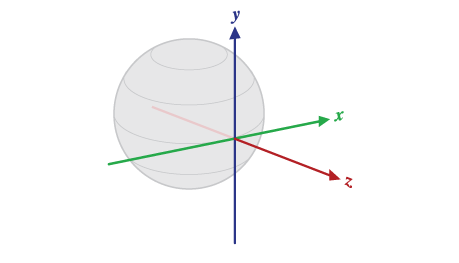
\includegraphics{Figuras/referencialterra.png}
    \caption{Referencia NED \\ Fonte: Documentação Android}
    \label{fig:referencialTerra}
\end{figure}{}

\subsection{Referencial do Veículo (Body Frame)}

Este referencial está fixo ao corpo e compreende a origem e orientação do objeto para qual a solução de navegação é utilizada. Assim sendo, a origem coincide com a origem do referencial local, no entanto os eixos são fixos em relação ao veículo. O eixo $z$ é normal ao solo; $y$ possui a mesma direção do movimento e $x$ completa o conjunto ortogonal.
Em termos do movimento angular: $z$ é o eixo de \textit{yaw}; $y$ o eixo de \textit{roll} e $x$ o eixo de \textit{pitch}

\section{Transferência de Coordenadas}

Dados dois referenciais inerciais

\begin{figure}
    \centering
    \subfloat[Vetores Alinhados.]{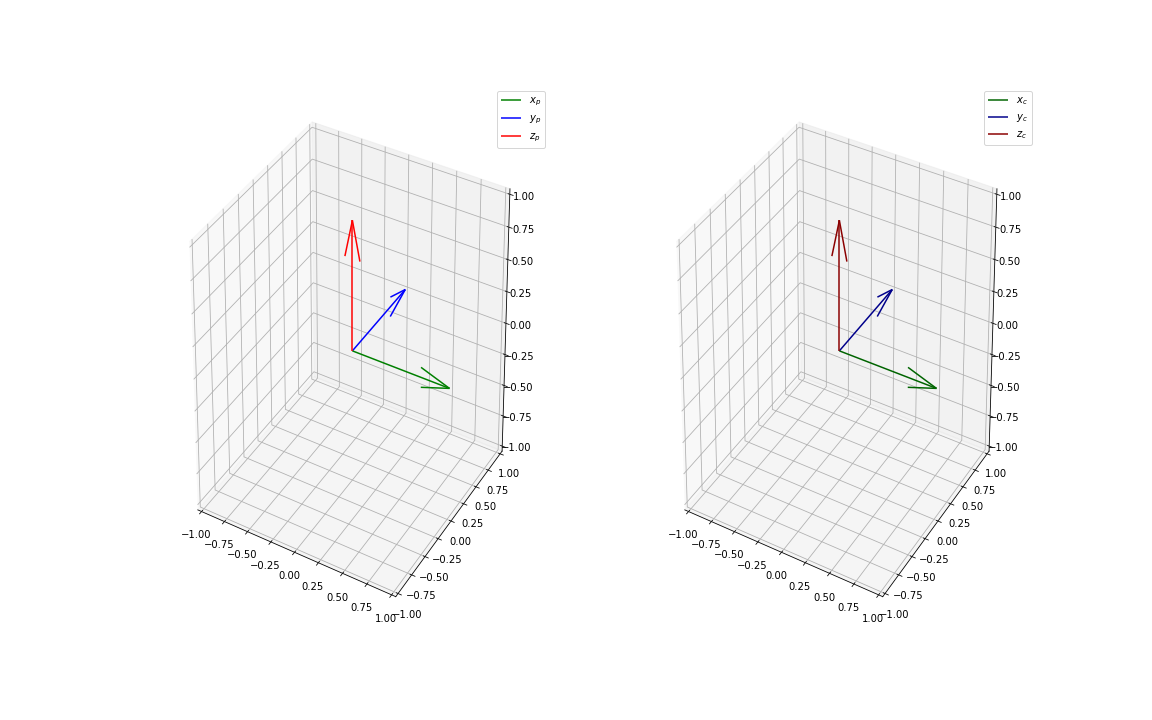
\includegraphics[height=70mm,width=\textwidth]{Figuras/alinhamentoDeVetores1.png}}
    \\
    \subfloat[Vetores com Eixos Invertidos.]{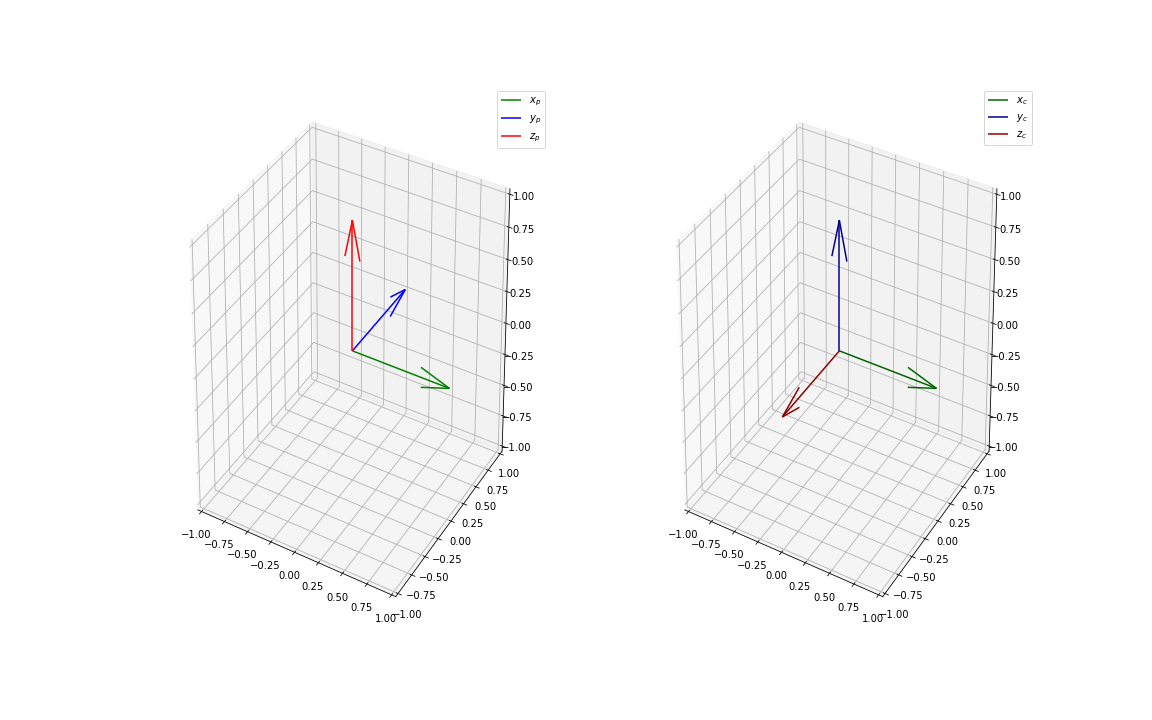
\includegraphics[height=70mm,width=\textwidth]{Figuras/alinhamentoDeVetores2.png}}
    \\
    \subfloat[Vetores caso Genérico.]{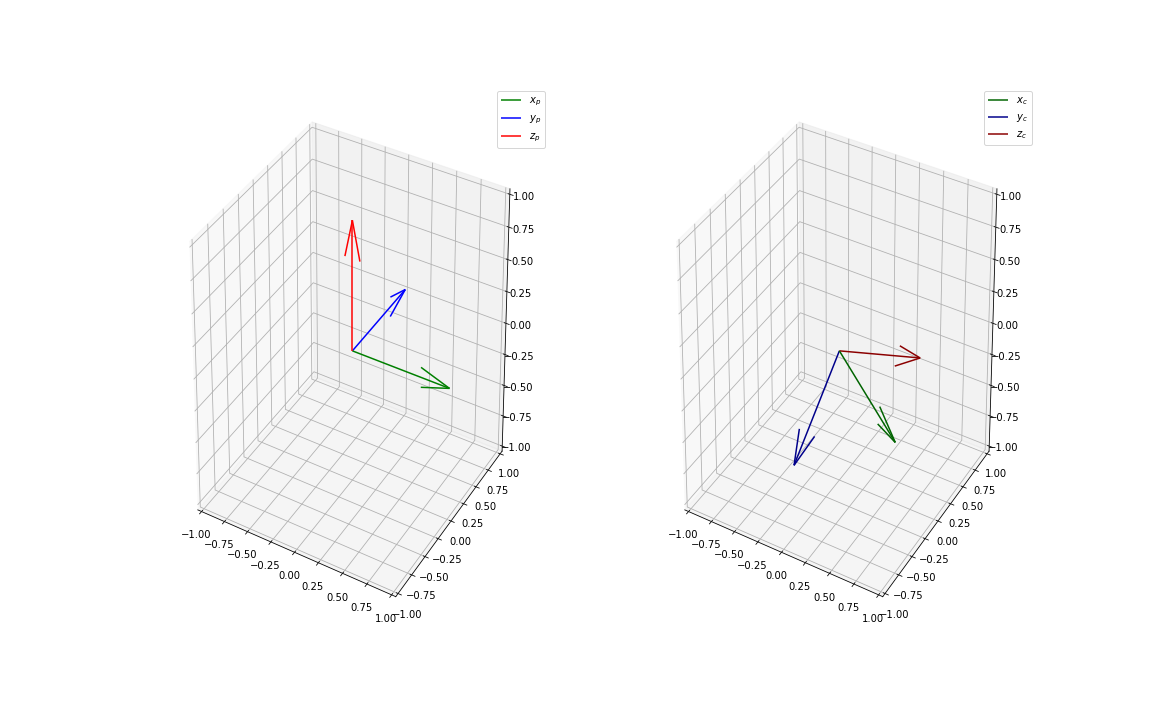
\includegraphics[height=70mm,width=\textwidth]{Figuras/alinhamentoDeVetores3.png}}
    \caption{Alinhamento de Vetores}
    \label{fig:alinhamentoDeVetores}
\end{figure}{}

\begin{equation} 
A_c = 
    \begin{bmatrix}
X_c\\ 
Y_c\\ 
Z_c
\end{bmatrix} e, A_p = 
    \begin{bmatrix}
X_p\\ 
Y_p\\ 
Z_p
\end{bmatrix}
\end{equation}{}

a transformação da base entre eles se dá por meio de uma matriz da forma:
\begin{equation}
    A_c = T . A_p
    \label{eq:equaçaoDaRotacao}
\end{equation}{}

onde:
\begin{equation}
    T = \begin{bmatrix}
T_{x_i} & T_{x_j}  & T_{x_k} \\ 
T_{y_i} & T_{y_j}  & T_{y_k} \\ 
T_{z_i} & T_{z_j}  & T_{z_k}
\end{bmatrix}
\end{equation}{}

Observando a Figura \ref{fig:alinhamentoDeVetores}(a) fica claro que a matriz de rotação nesse caso é a Identidade. Tal relação é tipicamente relevante quando se aborda o problema da transformação de base de um celular dentro de um veículo. Visto que, tomando a base $A_c$, como o sistema de coordenadas do carro. $y$ representaria movimentos de aceleração e desaceleração do veículo (aceleração longitudinal), $x$ representaria acelerações laterais e $z$ elevações. Tal percepção permite derivarmos a matriz de rotação para qualquer posição dentro de um veículo contanto que saibamos as direção da aceleração para frente e a gravidade. Como por exemplo no caso da Figura \ref{fig:alinhamentoDeVetores}(b) onde a matriz de rotação é :

\begin{equation}
    T = \begin{bmatrix}
1 & 0  & 0 \\ 
0 & 0  & -1 \\ 
0 & 1  & 0
\end{bmatrix}
\end{equation}{}

que aplicando na Equação \ref{eq:equaçaoDaRotacao} para esse caso em específico tem-se:

\begin{equation}
\begin{bmatrix}
1 & 0  & 0 \\ 
0 & 1  & 0 \\ 
0 & 0  & 1
\end{bmatrix} = 
\begin{bmatrix}
1 & 0  & 0 \\ 
0 & 0  & -1 \\ 
0 & 1  & 0
\end{bmatrix}
\begin{bmatrix}
1 & 0  & 0 \\ 
0 & 0  & 1 \\ 
0 & -1  & 0
\end{bmatrix}
\end{equation}{}


De modo que $T_{\hat{i}}$ representa a aceleração lateral sentida pelo celular, $T_{\hat{j}}$ representa a aceleração longitudinal, e $T_{\hat{k}}$ representa a Normal.
A partir disso, é possível se gerar uma matriz de rotação para uma posição genérica do celular contanto que se saiba a direção das acelerações.




\section{Orientação do Veículo}
A forma mais comum de estimar a orientação de um veículo é se utilizando de um sistema global de navegação por satélite (GNSS)\cite{almazan2013full}, como o GPS, por exemplo. 

A direção do carro pode ser medida através de dois GPS(frontal e traseiro) ou calculando-se a diferença entre dois pontos consecutivos. A priori, esse método de posicionamento possui diversas limitações: A frequência máxima é aproximadamente 1 $Hz$; isso significa que a 60 $Km/h$, um veículo teria se deslocado 20m da sua posição inicial. Ainda devido a baixa frequência, não se é possível captar movimentos bruscos em uma viagem comum de carro, que ocorrem em frações de segundos. Ressalta-se \cite{almazan2013full} que esse tipo de monitoramento não funcionam sob baixa visibilidade de satélites (tuneis e viadutos em geral).

Li \cite{li2009vehicle} utilizou a fusão de sensores, baseada em um sistema de observador de cascata e foi capaz de estimar a direção e velocidade do veículo inclusive durante manobras complexas, com elevada acurácia. Tendo-se em vista que informações como o angulo do volante, e a pressão realizada nos pedais do veículo são diretamente relacionados com o dinâmica do sistema. 

Com o proposito de lançar mão desse tipo de informação a respeito do veículo (que é transmitida através do protocolo bus-CAN) diversas pesquisas utilizam um conector OBD-II de forma a coletar os dados. A grande vantagem desse método consiste em aumentar em atingir uma frequência mais de 1 $Hz$ não limitada ao campo aberto para estimar o estado do veículo. No entanto existem duas contra-indicações. Primeiramente, se trata de um método invasivo que obriga o usuário a plugar um novo dispositivo no veículo. Segundamente, cada fabricante de veículo possui seu próprio protocolo \cite{almazan2013full} e todos deveriam ser conhecidos previamente para arquitetar uma solução barata e genérica.

Assim sendo, um método adotado para medir a dinâmica veicular, têm sido o uso de dispositivos portáteis, que se utilizam de uma combinação da medição do campo magnético da terra (através de um magnetômetro) e um outro sensor, como o GPS ou algum sensor inercial.
Existem alguns trabalhos (\citep{zheng2016unsupervised}, \citep{zheng2015mobileutdrive},\citep{almazan2013full}) na literatura que utilizam-se dessa combinação para se estimar a orientação de um smartfone no interior de um veículo. A vantagem desse método advém do aumento da frequência de captura de dados. Porém é um método significantemente influenciado por interferência de campos magnéticos \cite{almazan2013full}. Nesse sentido, a sensibilidade do magnetômetro é alta e devido a grande quantidade de componentes eletro-mecânicos no veículo, seu comportamento é altamente comprometido. 

Além disso, existem trabalhos que buscam utilizar a fusão de sensores inerciais (IMU) e GNSS para superar as limitações já mencionadas a respeito dos GNSS. Todavia, a orientação de um IMU no veículo deve ser conhecida anteriormente, de forma a se obter medições condizentes com a dinâmica do veículo.

Em linhas gerais, é necessário saber a posição do smartfone em relação ao sistema de coordenadas do veículo para que se possa combinar os sensores inerciais com o GNSS.

\citet{you2013carsafe} Propôs um aplicativo que visa alertar o motorista desatento, através da utilização de duas câmeras. \citeauthor*{bergasa2014drivesafe}\citep{bergasa2014drivesafe} propuseram um aplicativo que também possui como objetivo alertar desatenção e pontuar o motorista utilizando visão computacional, em conjunto com sensores IMU do smartfone, GPS e o microfone do aparelho. Em ambos os casos os autores se utilizam do aparelho fixo de forma a realizar a fusão de sensores. A solução proposta por esses autores, busca imitar algumas funcionalidades encontradas em diversos veículos top de linha no mercado. Ainda assim se apresentando como uma alternativa as "caixas-pretas" fornecidas, muitas das vezes, por seguradoras.

\citeauthor{chen2015d} argumenta em seu trabalho que ao monitorar o comportamento anormal de direção é possível conscientizar o motorista dos seus próprios hábitos. Uma vez que grande parte dos motoristas são autoconfiantes e não estão cientes de seus comportamentos agressivos. Ao identificar os hábitos ruins de direção automaticamente, o motorista pode tornar-se consciente de seu comportamento e então corrigi-lo. Assim podendo evitar futuros acidentes em potencial. Com isso em vista, \citeauthor{chen2015d} foi capaz de usar SVM para detectar 6 manobras de direções, a partir de 16 características extraídas com base em 6 meses de corridas coletadas. Todas as viagens foram realizadas com o celular alinhado com o carro.

\citeauthor{eren2012estimating} por sua vez foi capaz de classificar estilos de direção utilizando IMU e dados de GPS. Através de um algortimo de DTW, para compensar as diferenças temporais dos eventos. Da mesma forma que \citeauthor{fazeen2012safe} contribuiu com um sistema de monitoramento do comportamento do motorista que o avisa na ocorrência de manobras perigosas. Entretanto ambos os sistemas dependem do alinhamento do smartfone com o veículo, de modo a extrair as informações corretas dos sensores.

Com o objetivo de alinhar o sistema de coordenadas do aparelho celular com o carro \citeauthor*{dai2010mobile}\citep{dai2010mobile} sugeriram uma calibração baseada em IMU para obter os ângulos de "\textit{roll}" e "\textit{pitch}" do smartfone. No entanto, foi assumido que o smartfone estava alinhado com o eixo longitudinal do veículo; ou seja o ângulo de "\textit{yaw}", nesse caso, deve ser nulo. De forma análoga \citeauthor{almazan2013full} propôs um método de auto-calibração que estima o ângulo de "\textit{yaw}" do smartfone, em relação ao veículo para o celular em uma posição genérica.

\citeauthor{castignani2015driver}, por outro lado, propôs um sistema \textit{fuzzy} para monitorar o comportamento do motorista onde a direção é classificada como calma ou agressiva. No estudo em questão, foi levada em consideração a magnitude do vetor aceleracão de forma a mitigar o problema de decompor a aceleração lateral e logitudinal.


 
\section{Detecção de Manobras}

\citeauthor{fazeen2012safe} Através do seu método de monitoramento proposto, estudou os padrões de direção utilizando um celular Nexus One em diversos cenários. Com isso ele foi capaz de demonstrar os padrões seguros e repentinos de diversas manobras. De acordo com Autor \citep{fazeen2012safe}, acelerações e desacelerações seguras nunca atingem uma força g maior que $\pm 0.3g $ (aproximadamente $3m/s^2$); já as manobras bruscas chegam a $\pm 0.5g$ (aproximadamente $5m/s^2$).

\citeauthor*{Paefgen:2012:DBA:2406367.2406412} de forma similar, foram capazes de criar uma aplicação mobile que avalia o comportamento do motorista com base em medições do acelerômetro que fornece de forma instantânea informações a respeito da qualidade da direção do motorista. De forma a buscar validação, eles compararam os eventos registrados pelo smartfone com os eventos medidos em um IMU fixo no veículo, em um estudo de campo controlado. Por fim os autores identificaram que os smartfones tendem a sobreestimar eventos críticos de direção.

Outra contribuição interessante partiu de \citeauthor{zheng2015mobileutdrive} (\citeyear{zheng2015mobileutdrive}) que mostrou que a velocidade angular observado no eixo $z$ de um dispositivo alinhado com o carro, possui elevada correlação com o ângulo do volante. 


\chapter{Metodologia} \label{Metodologia}

Neste capítulo será apresentada a formulação geral do problema de Transferência de Coordenadas, bem como a solução proposta para detecção das manobras realizadas em uma corrida.

\section{Formulação do Problema e metodologia}

Trabalhos anteriores (citar) que se utilizaram de smartfones para realizar a coleta de informações a respeito do comportamento do motorista, não levaram muito em consideração a calibração correta dos eixos do aparelho com o carro. Muitas das vezes, Lançando-se mão de que para descrever os padrões de direção de um veiculo, o alinhamento manual do eixo do telefone, para com o do veículo pode ser suficiente. No entanto, o objetivo do presente trabalho consiste em aplicar um método consistente para se obter a detecção de manobras independente da posição do celular no carro. Nesse sentido uma troca de bases se faz necessária.

Definiu-se o cenário de aplicação de que para cada viagem, o aparelho celular pode estar posicionado em qualquer desconhecido, no entanto fixo.

\section{Transferência de Coordenadas}

A principio não se pode compreender a dinâmica veicular através da leitura de sensores, a não ser que o sistema de coordenadas do telefone esteja alinhado com o do veículo. A princípio se propõem em realizar o alinhamento dos eixos utilizando o giroscópio e o acelerômetro.

O sistema de coordenadas do telefone ($X_t,Y_t,Z_t$) é determinado pela posição do mesmo, no interior do veículo. O alinhamento do coordenadas consiste em encontrar a matriz de rotação que alinha o sistema de coordenadas do telefone com o do Veículo ($X_v,Y_v,Z_v$). 

Primeiramente, define-se um vetor unitário de três coordenadas no sistema de coordenadas do veículo, $\hat{i}$,$\hat{j}$ e $\hat{k}$.(por exemplo com $\hat{i} = [1,0,0]$ no sistema de coordenadas do veículo). Denotamos as coordenadas correspondentes desse vetor unitário no sistema de coordenadas do telefone como:

\begin{equation}
    \hat{q} = [x_q,y_q,z_q]
\end{equation}{}

onde $\hat{q} \in i,j,k$  dessa forma a matriz de rotação é dada por:

\begin{equation}
    R = \begin{Bmatrix}
x_i &x_j  &x_k \\ 
y_i &y_j  &y_k \\ 
z_i &z_j  &z_k 
\end{Bmatrix}
\end{equation}{}

Para se obter cada elemento da matriz de rotação, utilizamos medições de acelerômetro e do giroscópio.

\subsection{Derivando Aceleração Gravitacional} 
Pode ser obtido utilizando um filtro de passa-baixa(exemplo: suavização exponencial) nos três eixos do acelerômetro para se obter as componentes constantes nesses três eixos, de forma a se encontrar a gravidade, atuante sobre o smartfone. Essa medição é realizada nos primeiros instantes em que o celular se encontra parado. Então é possível obter-se a média dos três eixos que é então normalizada de forma a gerar o vetor unitário $\hat{k} = [x_k,y_k,z_k]$  

\begin{figure}
    \centering
    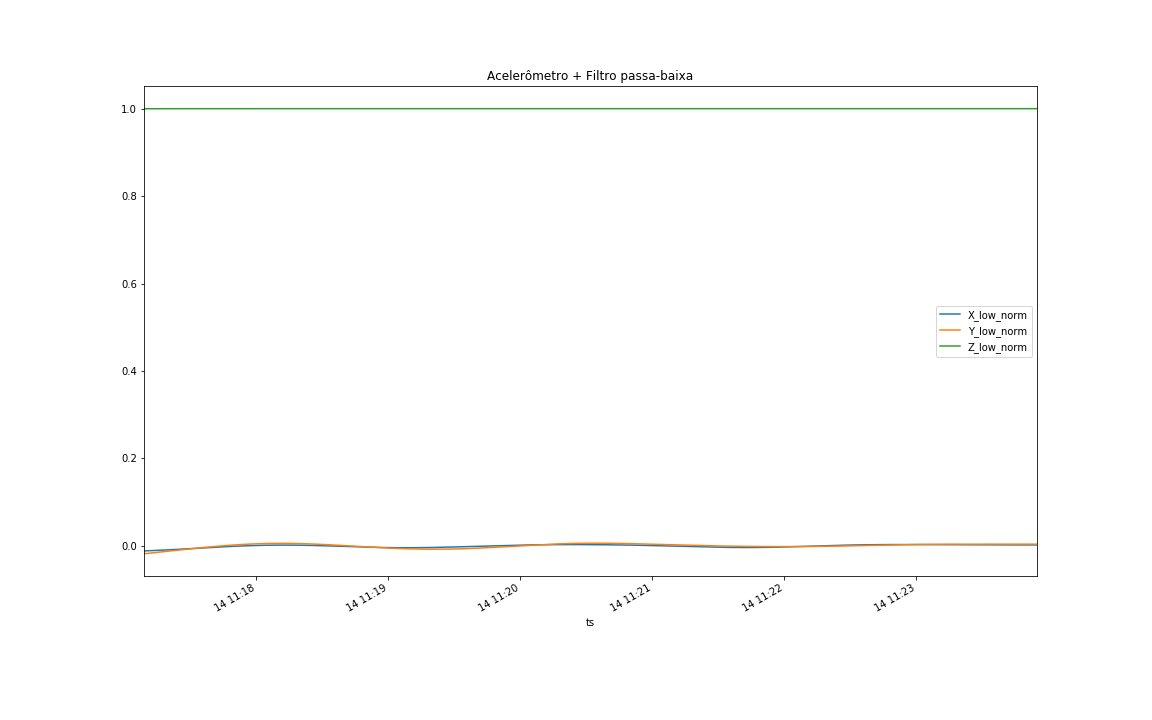
\includegraphics[width=150mm]{Figuras/acelerometroPassaBaixa.png}
    \caption{Medições dos três eixos do Acelerômetro após aplicação do filtro passa-baixa. }
    \label{fig:acelerometroPassaBaixa}
\end{figure}

\subsection{Derivando Aceleração Longitudinal}
Para se obter $\hat{j}$ lançamos mão do fato de que as leituras nessa direção de movimento do veículo são dadas quando aceleramos ou desaceleramos com o carro em linha reta. Quando o celular é colocado no painel do veículo ou montado em algum suporte, com o carro ligado, ele é submetido a um determinado nível de vibração, que varia de veículo para veículo. Quando se acelera em linha reta, os primeiros micro segundos dessa aceleração longitudinal pode ser observada em termos da magnitude da aceleração linear. que, nesse momento, é essencialmente um vetor que aponta na direção do movimento do carro, e tipicamente maior do que o ruido observado quando o carro ainda se encontra em repouso. 

Em vista da característica ruidosa do acelerômetro, Não é possível estimar o vetor velocidade - que possui o mesmo sentido do movimento do carro - com acurácia; o erro numérico da integração se acumula de forma rápida, tornando a medição imprecisa. No entanto, a direção do vetor velocidade pode ser estimada através dessa integração, e por mais que o erro numérico mascare o valor real da velocidade, sua direção continua condizente com a direção de movimento do veículo. Para o calculo da integral, podemos utilizar o giroscópio para determinar se o veículo está se locomovendo em linha reta; nesse caso a magnitude do giroscópio é muito próxima de zero, e em seguida encontramos o instante onde o veículo acelera, encontrando $\hat{j} = [x_j,y_j,z_j]$. De acordo com (citar autor) deve-se excluir a componente da gravidade que pode se distribuir em todos os três eixos do telefone, dessa forma tornando o modelo robusto ao plano inclinado.



\begin{figure}
    \centering
    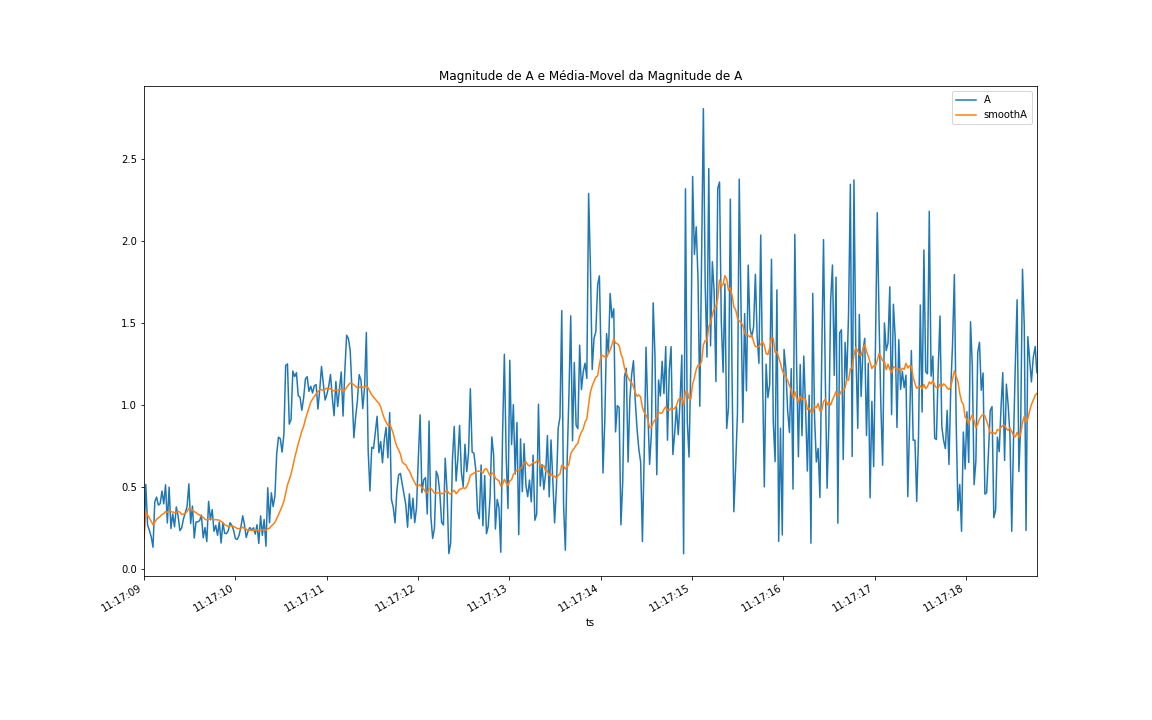
\includegraphics[width=150mm]{Figuras/acelerometroMediaMovel.png}
    \caption{Magnitude da Aceleração Linear com e sem filtro de passa-baixa}
    \label{fig:acelerometroMediaMovel}
\end{figure}

\subsection{Derivando Aceleração Lateral}
Como o sistema de coordenadas segue a regra da mão direita, $\hat{i} =\hat{j} \times \hat{k} = [x_i,y_i,z_i]$.

Depois de se obter a matriz de rotação $R$ Nós podemos obter a leitura dos sensores \begin{equation}
    s^{'} = s \times R \label{eq:trocaDeBase}
\end{equation}

 Deve-se frisar que, o escopo do presente trabalho não contempla o caso onde o dispositivo se encontra não fixo no carro (ex.: na mão do motorista). Quando é detectada algum pico na magnitude do giroscópio maior do que o limiar de 1.5 rad/s, o aparelho deve ser considerado como descalibrado e a transferência de coordenadas deve ser reestimada. Uma vez que um pico dessa magnitude pode representar que a posição do telefone foi alterada. Dado que a média magnitude do giroscópio se mantém próximo a 0 na maior parte da viagem chegando a 0.5-0.6 rad/s em momentos de curva.


\section{Teste da Transferência de Coordenadas no Conjunto de Dados Aberto}
A fim de se confirmar o método de transferência de coordenadas proposto se utilizou, a princípio, os dados coletados em trabalhos anteriores \cite{junior2017driver}. O conjunto de dados coletados em questão consiste em 4 viagens experimentais de aproximadamente 13 minutos cada, onde se executaram diversas manobras agressivas de direção. Para tal experimento foi-se utilizado o veículo Honda Civic 2011. Para captura de dados utilizou-se um aparelho Motorola XT1058 com Android versão 5.1. O aparelho em questão foi fixado no para-brisa do veículo durante a viagem, por meio de um suporte, e o mesmo não foi movido ou operado durante a captura dos sensores. A taxa de amostragem dos sensores variou entre 50 a 200 Hz, a depender do sensor. Os carros foram dirigidos por dois motoristas com 15 anos de experiência. O dia em que o experimento ocorreu era ensolarado. Ressaltando-se que os dados coletados de acelerômetro e giroscópio neste experimento estavam no sistema de coordenadas Global; ou seja, o eixo Z apontando para o centro da terra, Y para o norte magnético e X sendo ortogonal aos dois primeiros.

Para se obter as medições da aceleração linear e da gravidade atuante sob o smartfone, utilizou-se respectivamente um filtro passa-alta e um filtro passa-baixa. Permitindo-se assim a obtenção dos sensores "virtuais".

Com isso, buscou-se identificar os momentos em que a magnitude da velocidade angular, medida pelo giroscópio, era baixa; ou seja, o aparelho se encontrava essencialmente parado, e um pico da magnitude da aceleração linear - nesse caso, suavizada com uma média móvel - que estivesse 2 vezes acima do patamar registrado antes de iniciar o movimento do carro \ref{fig:janelaCalibracao}.

\begin{figure}
    \centering
    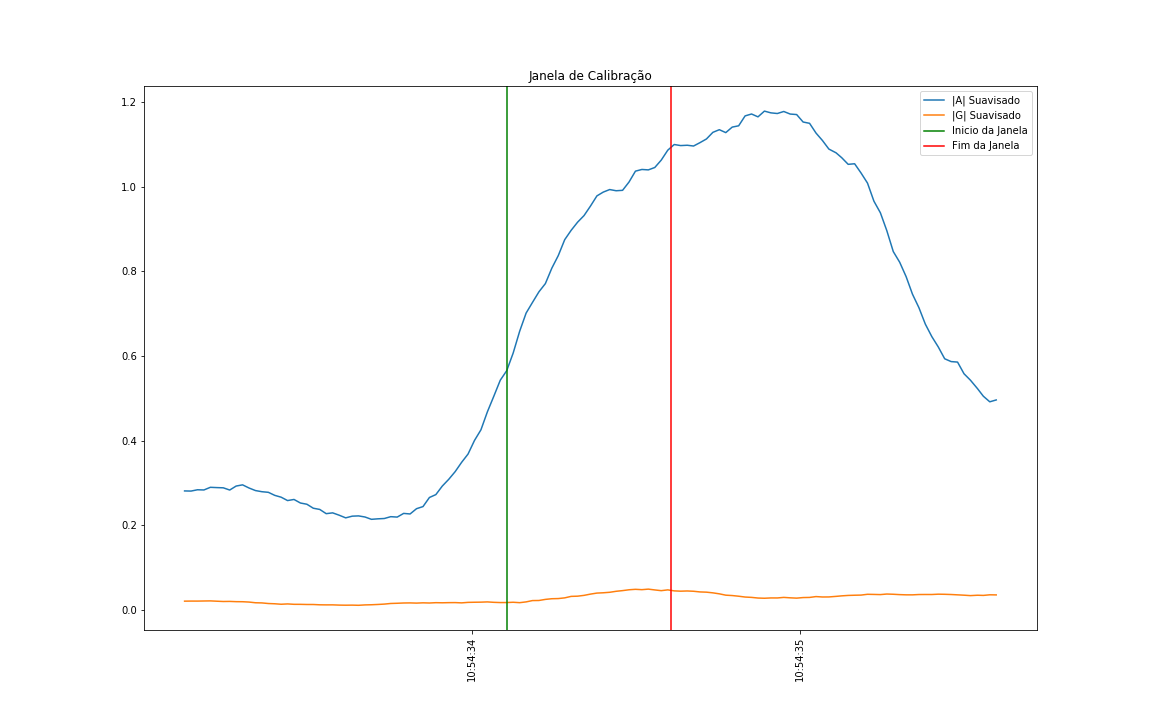
\includegraphics[width=150mm]{Figuras/janelaCalibracao.png}
    \caption{Janela em que os dados para gerar a matriz de rotação são capturados.}
    \label{fig:janelaCalibracao}
\end{figure}

Desse momento se inicia uma janela de 500ms. Ao fim da janela são estimados $\hat{i}$,$\hat{j}$,$\hat{k}$, por fim gerando a matriz de rotação. Em seguida as medições de acelerômetro linear e giroscópio, são transformadas utilizando-se a matriz, de acordo com a equação \eqref{eq:trocaDeBase}.

\begin{figure}[H]
    \centering
    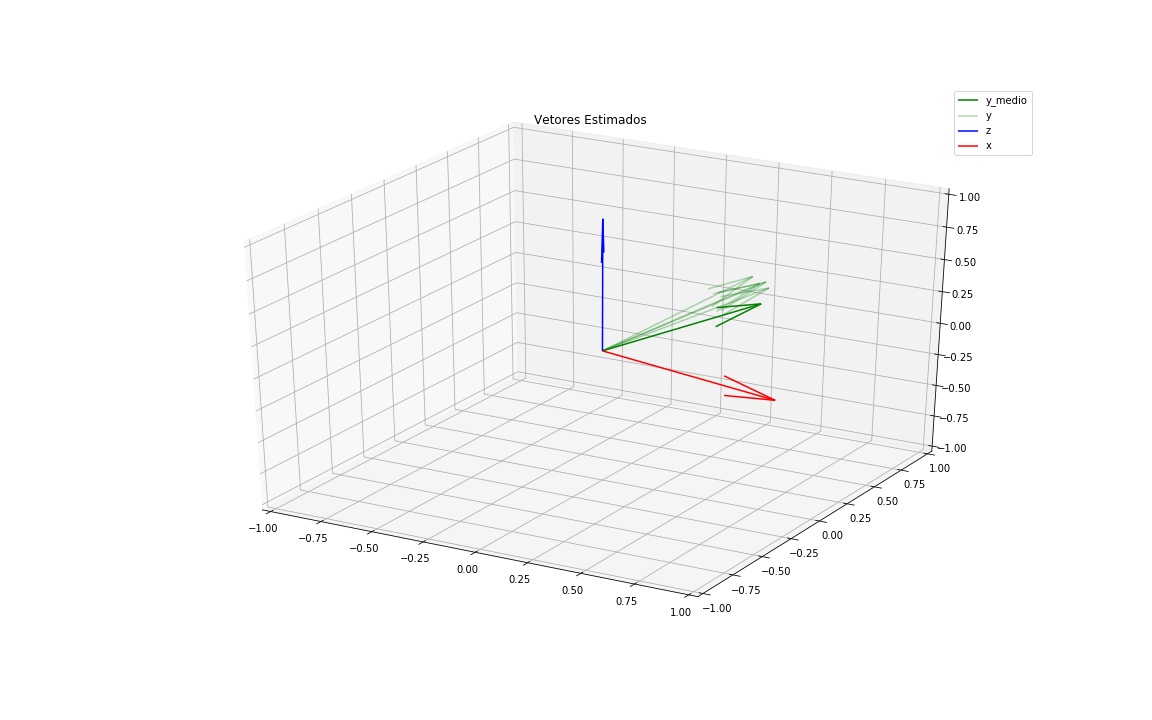
\includegraphics[width=150mm]{Figuras/vetoresEstimados.png}
    \caption{Vetores estimados para matriz de rotação.}
    \label{fig:vetoresEstimados}
\end{figure}{}

\begin{figure}[H]
    \centering
    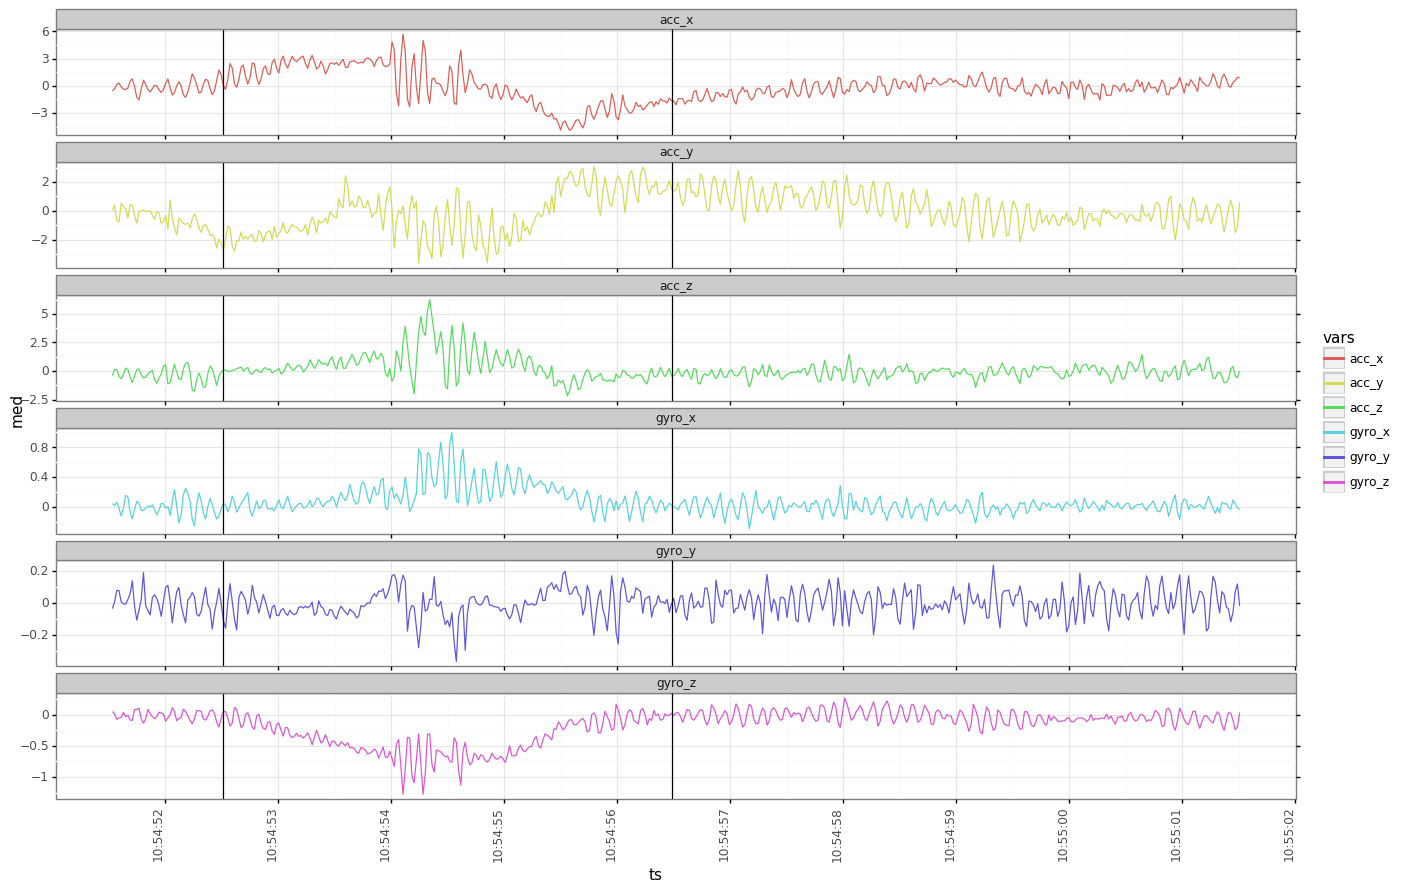
\includegraphics[height=110mm]{Figuras/assinaturaCurvaDireita.png}
    \caption{Assinatura de Curva Direita com os dados de sensor rotacionados.}
    \label{fig:assinaturaCurvaDireita}
\end{figure}{}

\section{Teste da Transferência de Coordenadas no Conjunto de Dados Próprio}

Para um segundo experimento, dessa vez com dados próprios, se utilizou o aplicativo "Sensor Record" que permite a gravação de diversos sensores do dispositivo Android. No caso, utilizou-se um aparelho Xiaomi Mi 8 Lite, gravando os dados do sensor de giroscópio, acelerômetro linear e gravidade, presentes no dispositivo, a uma frequência de amostragem média de 100 Hz. O veiculo utilizado no experimento foi um Toyota Corolla 2005. Todas as viagens foram realizadas pelo mesmo motorista, com mais de 20 anos de experiência. Os dados foram gravados na parte do dia em uma corrida que compreendia um percurso de aproximadamente 1km. O smartfone foi disposto em 3 posições em termos do seu sistema de coordenadas como descrito a seguir e observado na Figura \ref{fig:posicoesCelular};

\begin{itemize}
    \item Alinhado com o veículo
    \item Deitado sob o painel com sua coordenadas X alinhada com a coordenada Y do carro
    \item Posição genérica
\end{itemize}{}

Nos três casos foi-se utilizado o método desenvolvido para se estimar a matriz de rotação. Que consiste em identificar o instante em que o veículo se encontra essencialmente parado, e monitorar a magnitude da aceleração sentida pelo aparelho. No momento em que essa magnitude for 2 vezes maior que a vibração normal do carro - registrada a partir dos primeiros instantes que o celular se encontra parado. Assim sendo, é possível integrar a aceleração por um período curto de tempo, com o objetivo de se estimar a direção do carro. Nesse momento também se toma a média do vetor gravidade atuante sobre o dispositivo. Por fim é possível se estimar uma matriz de rotação que transforma as coordenadas do celular para as coordenadas do carro.

\begin{figure}[h]
    \centering
    \subfloat[Posição 1 (Alinhado).]{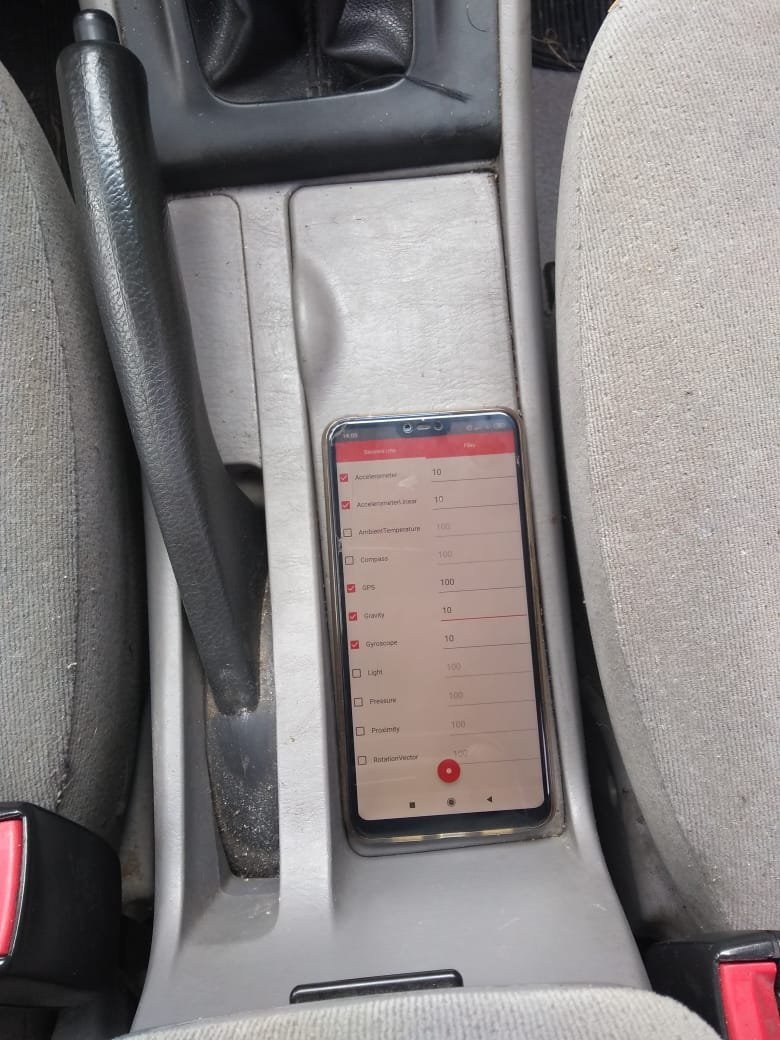
\includegraphics[width=0.3\textwidth]{Figuras/cellPosition1.jpeg}}
    \hfill
    \subfloat[Posição 2 (Deitado).]{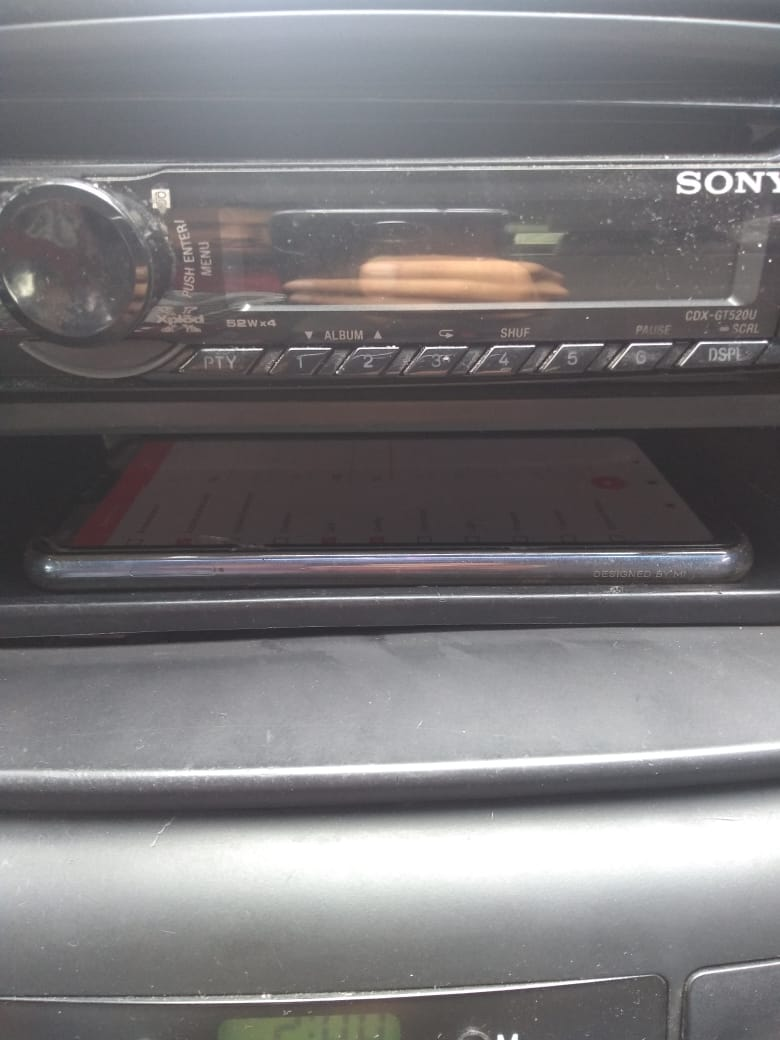
\includegraphics[width=0.3\textwidth]{Figuras/cellPosition2.jpeg}}
    \hfill
    \subfloat[Posição 3 (Genêrica).]{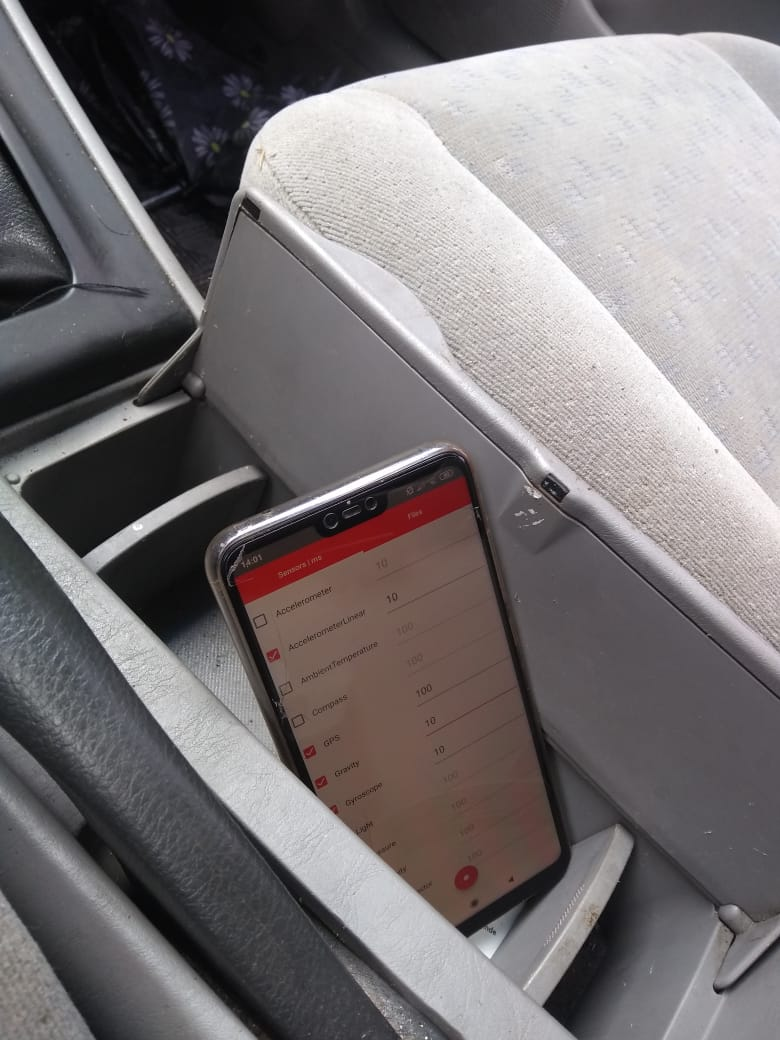
\includegraphics[width=0.3\textwidth]{Figuras/cellPosition3.jpeg}}
    \caption{Posições do Celular}
    \label{fig:posicoesCelular}
\end{figure}{}

De forma a se obter validação do método para troca de coordenadas, se observou: O coeficiente de correlação de Pearson dos dados rotacionados - no caso dos eixos conhecidos; a quantidade de energia em Y - uma vez que as corridas se deram no mesmo percurso e em condições muito parecidas, elas tendem a ser próximas; a direção das curvas, uma vez que o percurso consiste em uma volta em um quarteirão, haverão 4 assinaturas de curva para direita, tanto pelo eixo Z rotacionado do giroscópio, quanto pelo eixo X rotacionado do acelerômetro; dessa forma permitindo identificar se a troca de base foi ou não bem sucedida.



\chapter{Resultados}\label{Resultados}

Neste capítulo serão apresentados os resultados obtidos segundo a formulação dos Capítulos \ref{Transferência} e \ref{Metodologia}. Tais resultados serão discutidos e comentados, e também comparados com a literatura para obter-se validez.

\section{Troca de Coordenadas na posição 1 (Alinhado)}
No que diz respeito a posição do celular alinhado com as coordenadas do carro, foi observado a correlação alta (Figura \ref{fig:hmapTrip1}) entre os eixos. O que era esperado uma vez que a matriz de rotação nesse caso especifico se trata da matriz identidade. Ou seja, ao aplicada a matriz de rotação não deve haver alteração nas medições observadas.


\begin{figure}
    \centering
    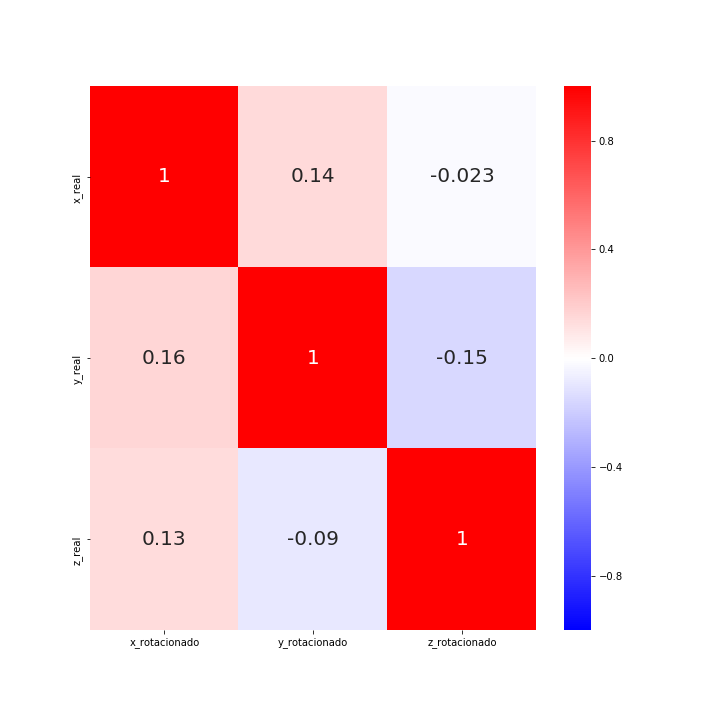
\includegraphics[width=100mm]{Figuras/hmaptrip1.png}
    \caption{Correlação entre os eixos, posição 1.}
    \label{fig:hmapTrip1}
\end{figure}{}
 
\begin{figure}
    \centering
    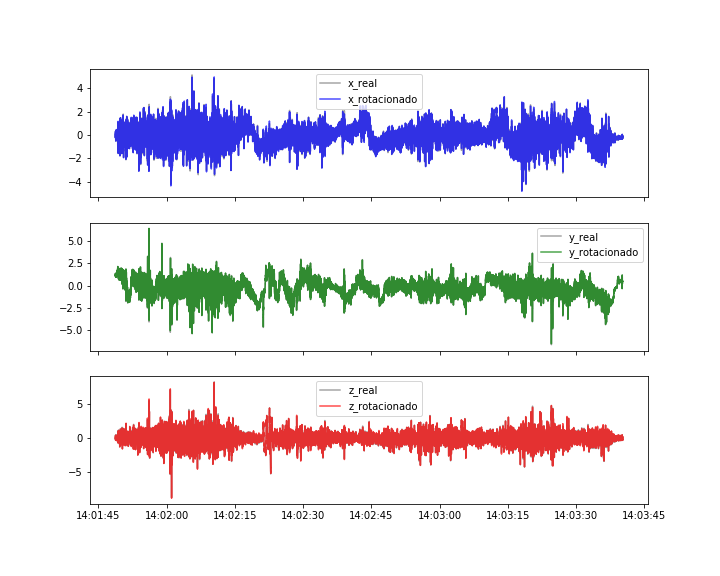
\includegraphics[width=150mm]{Figuras/realrotacionadotrip1.png}
    \caption{Correlação entre os eixos, posição 1.}
    \label{fig:realrotacionadoTrip1}
\end{figure}{}
 
\section{Troca de Coordenadas na posição 2 (Deitado)}
Para o caso do celular deitado, foi identificada uma correlação positiva entre o eixo X do aparelho e Y do carro; seguida de uma correlação negativa entre o X do carro e o Y do celular e positiva entre o eixo Z de ambos, conforme pode ser observado nas Figuras \ref{fig:hmapTrip2} e \ref{fig:realrotacionadoTrip2}.

\begin{figure}
    \centering
    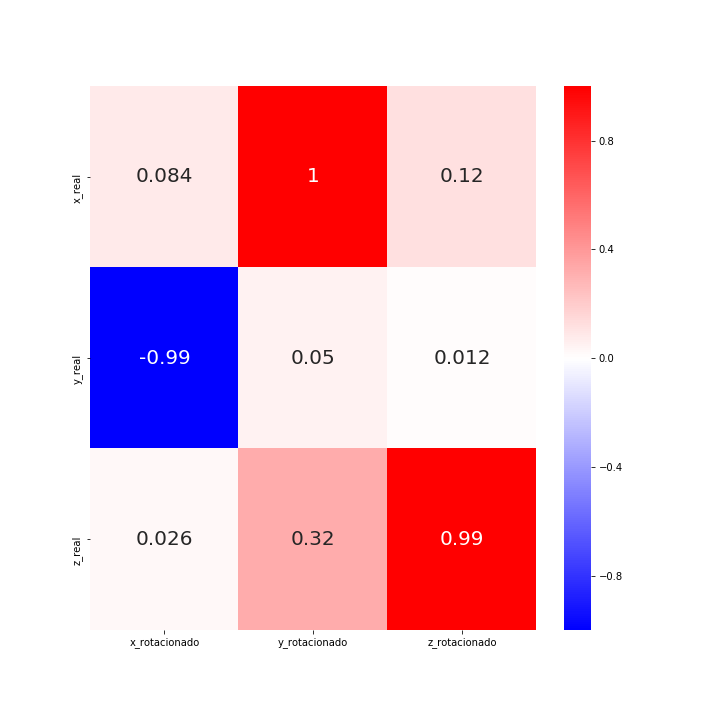
\includegraphics[width=100mm]{Figuras/hmaptrip2.png}
    \caption{Correlação entre os eixos, posição 1.}
    \label{fig:hmapTrip2}
\end{figure}{}
 
\begin{figure}
    \centering
    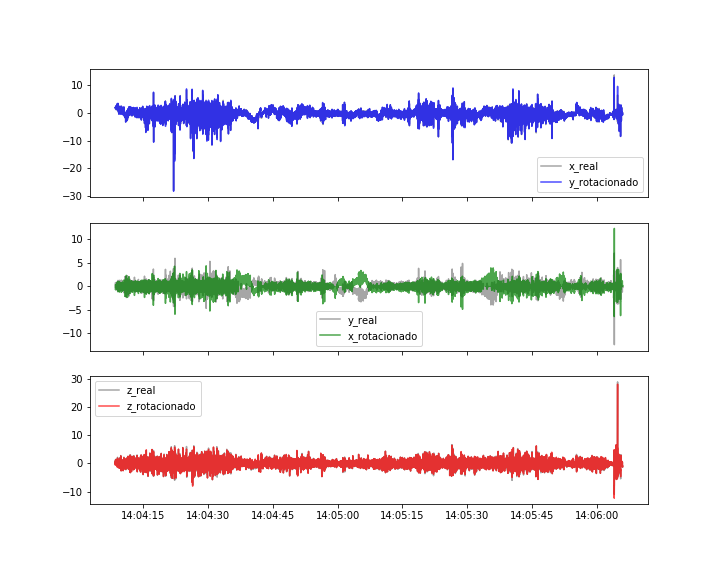
\includegraphics[width=150mm]{Figuras/realrotacionadotrip2.png}
    \caption{Correlação entre os eixos, posição 1.}
    \label{fig:realrotacionadoTrip2}
\end{figure}{}

\section{Troca de Coordenadas na posição 3 (Caso Genérico)}
Em termos do caso genérico, não é trivial observar se a rotação foi bem sucedida apenas observando-se a correlação entre os eixos. Nesse sentido, utilizou-se uma abordagem indireta. Onde, primeiramente se observou o quanto de energia (nesse caso em termos da variância) estava concentrada em cada eixo. Uma vez que o percurso foi o mesmo, e foi realizada em condições parecidas, os resultados do dado rotacionado devem convergir. Tal comportamento pode ser comprovado de acordo com a Tabela \ref{tab:qtdEnergiaPorEixo}. 


\begin{table}[]
\caption{Quantidade de Energia por Eixo Rotacionado}
\label{tab:qtdEnergiaPorEixo}
\begin{tabular}{cccc}
\hline
\textbf{Posição} & \textbf{\% Energia em X} & \textbf{\% Energia em Y} & \textbf{\% Energia em Z} \\ \hline
1 (Alinhado) & 31.42 & 63.98 & 4.60 \\
2 (Deitado) & 34.67 & 60.46 & 4.86 \\
3 (Genérico) & 28.78 & 63.61 & 7.61 \\ \hline
\multicolumn{4}{c}{Fonte: Próprio Autor a partir dos dados coletados}
\end{tabular}
\end{table}

No entanto, somente o quantidade de energia não basta, porque ela apresentaria a mesma proporção caso o sentido dos vetores estimado na matriz de rotação fosse contrário. Com isso em vista, lançou-se mão de o percurso em que se realizou o experimento ser conhecido. Nesse caso, existem 4 curvas a direita no percurso, e estas devem possuir assinaturas distintas tanto no eixo X do acelerômetro rotacionado quanto no eixo Z do giroscópio. 

Devido ao fato do giroscópio medir a velocidade angular no eixo. Ele vai apresentar sinal negativo em Z quando uma curva for para direita (sentido horário do carro) e positiva para esquerda (sentido horário). Por outro lado, no eixo X do acelerômetro (que se refere a aceleração lateral) o valor é positivo no caso de uma curva a direita e negativo para uma curva a esquerda.

Tal comportamento pode ser observado nas três corridas conforme explicitado pela Figura \ref{fig:assinaturaCurvas}. Assim confirmando que a troca de base foi realizada através do método proposto, de forma bem sucedida em todos os três casos.

\begin{figure}
    \centering
    \subfloat[Posição 1 (Alinhado).]{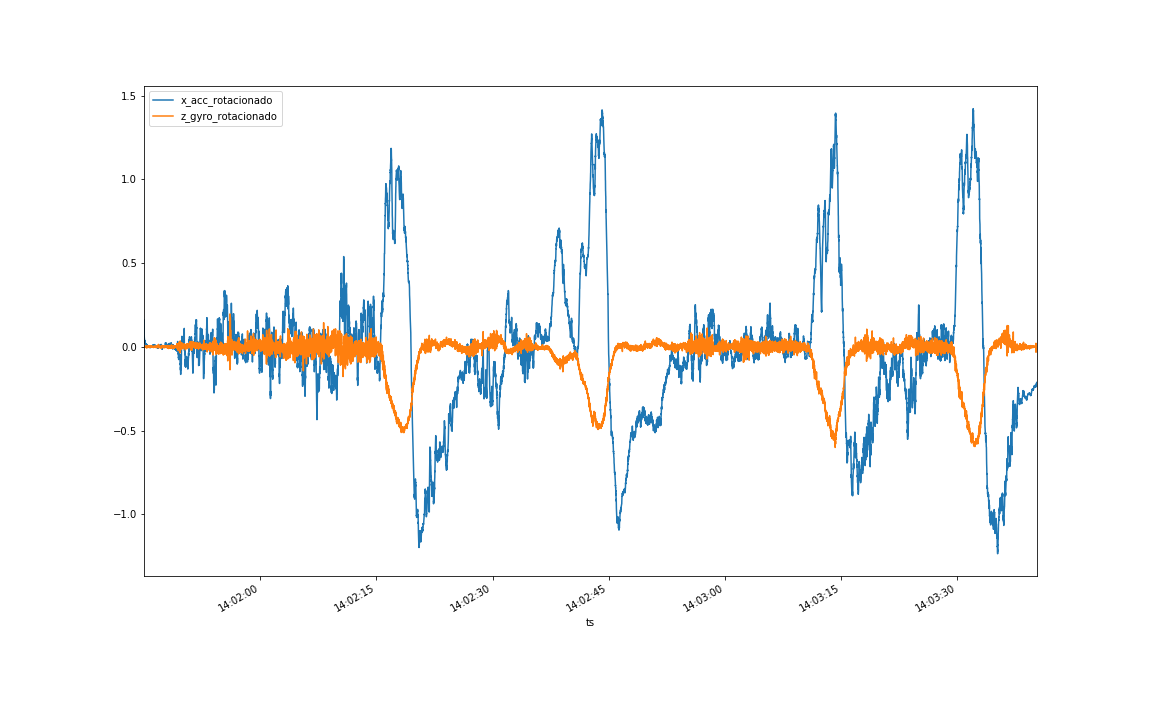
\includegraphics[height=50mm,width=\textwidth]{Figuras/curvaDireitatrip1.png}}
    \\
    \subfloat[Posição 2 (Deitado).]{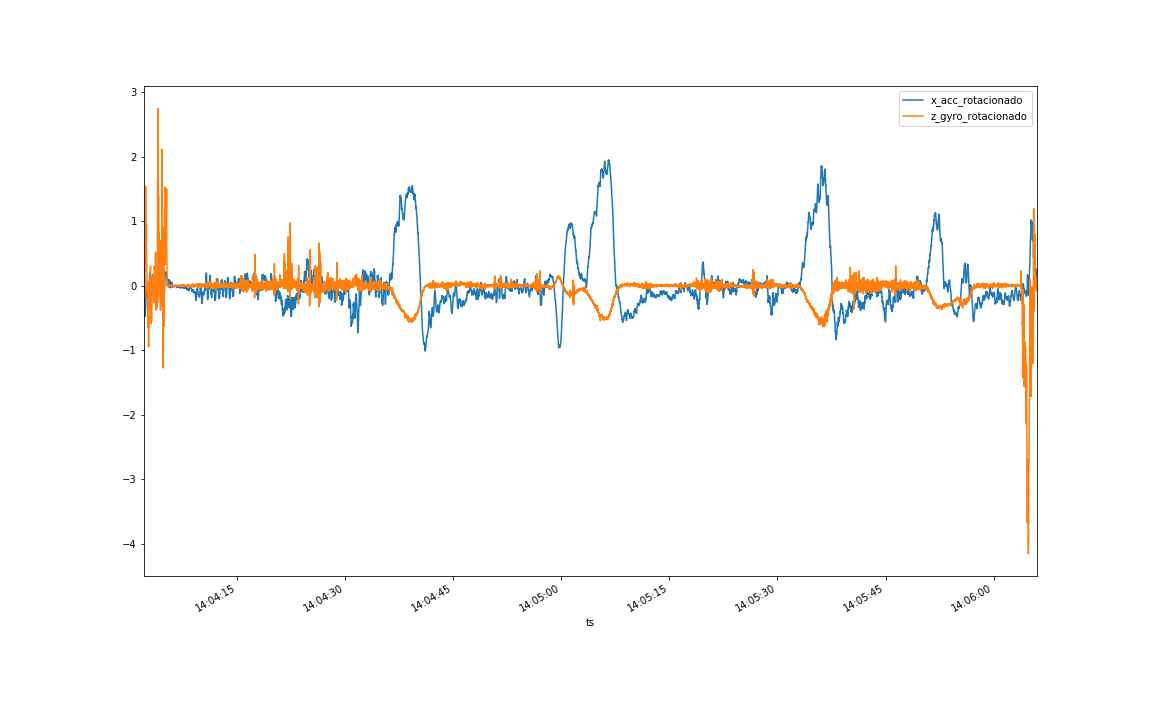
\includegraphics[height=50mm,width=\textwidth]{Figuras/curvaDireitatrip2.png}}
    \\
    \subfloat[Posição 3 (Genérica).]{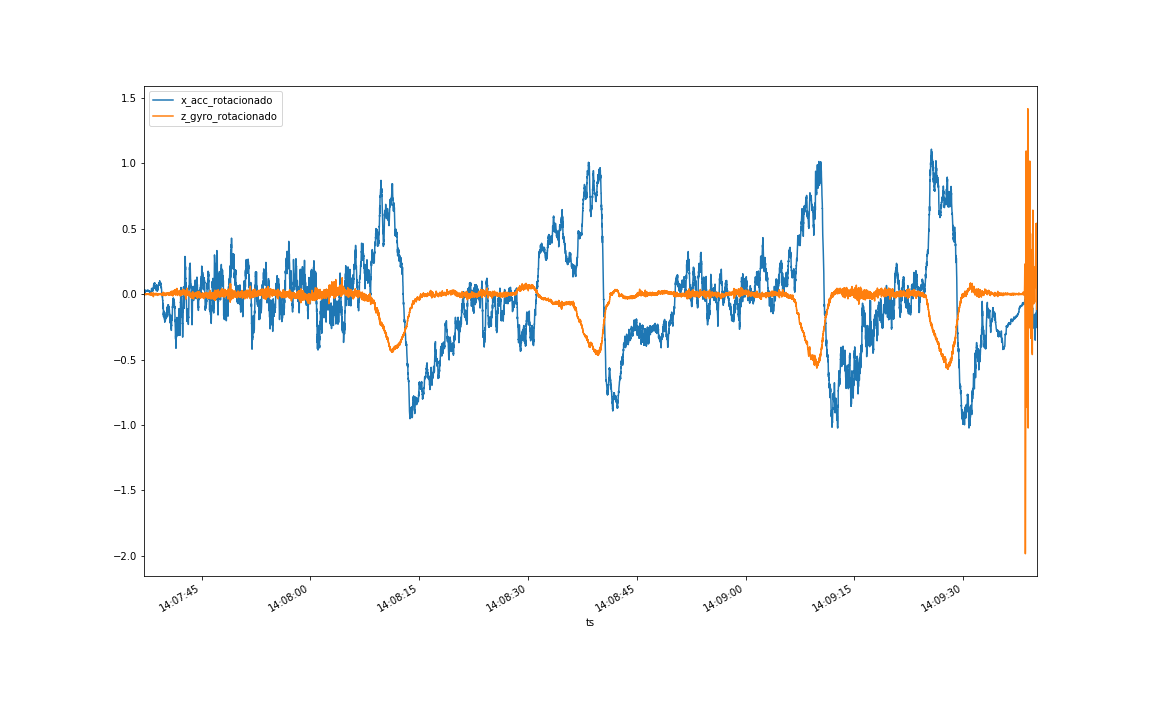
\includegraphics[height=50mm,width=\textwidth]{Figuras/curvaDireitatrip3.png}}
    \caption{Assinatura de curva nas diferentes posições}
    \label{fig:assinaturaCurvas}
\end{figure}{}

\citeauthor{zheng2016unsupervised} afirma que em estudos naturalísticos de direção, as manobras são geralmente anotadas manualmente e avaliadas de forma subjetiva através da revisão de vídeos. 

Uma vez que se possui o dado rotacionado, esse tempo pode ser reduzido através da detecção de eventos simples de direção.

Com o dado rotacionado, pode-se enfim, conforme visto em trabalho anteriores (\citep{zheng2016unsupervised}, \citep{Paefgen:2012:DBA:2406367.2406412} , \cite{fazeen2012safe}) através de limiares heurísticos, detectar eventos simples a respeito das corridas, de forma não supervisionada, facilitando assim o trabalho de classificação. 

De forma a realizar esse classificação não supervisionada, se utilizou os limiares presentes em \citep{Paefgen:2012:DBA:2406367.2406412} em conjunto com a conclusão de \cite{zheng2015mobileutdrive} a respeito da correlação alta entre o giroscópio e o manobrar do volante. De tal maneira que se pode classificar corretamente curvas, acelerações e desacelerações em todos os três casos (Figuras \ref{fig:eventosTrip1},\ref{fig:eventosTrip2},\ref{fig:eventosTrip3}).

\begin{figure}
    \centering
    \subfloat[Eventos no eixo $y$ do acelerômetro rotacionado.]{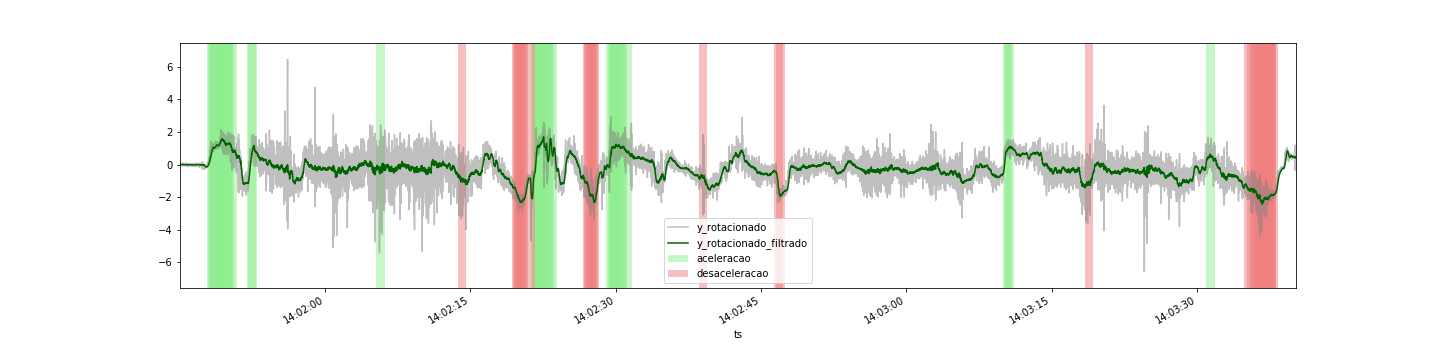
\includegraphics[height=70mm,width=\textwidth]{Figuras/eventosYtrip1.png}}
    \\
    \subfloat[Eventos no eixo $x$ do acelerômetro rotacionado e $z$ do giroscópio rotacionado.]{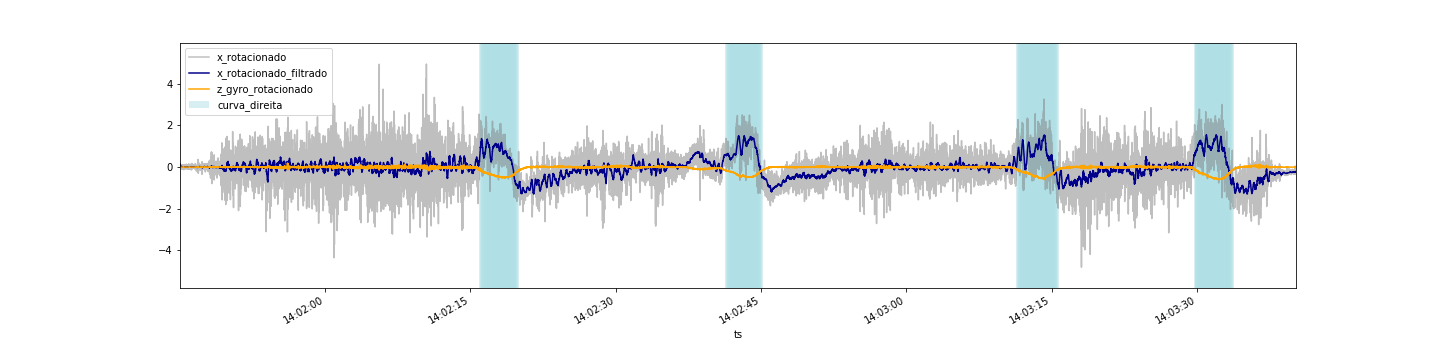
\includegraphics[height=70mm,width=\textwidth]{Figuras/eventosXGtrip1.png}}
    \caption{Assinatura de Eventos - Posição 1}
    \label{fig:eventosTrip1}
\end{figure}{}

\begin{figure}
    \centering
    \subfloat[Eventos no eixo $y$ do acelerômetro rotacionado.]{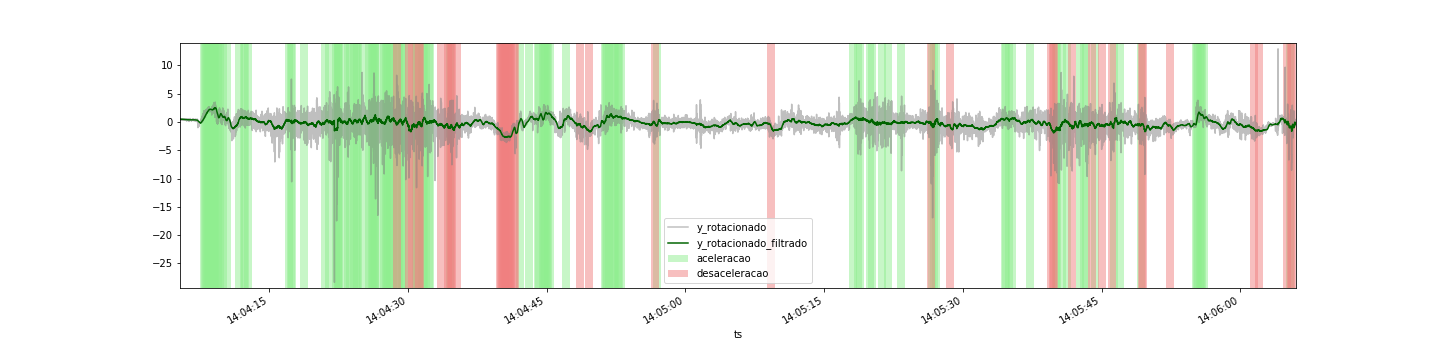
\includegraphics[height=70mm,width=\textwidth]{Figuras/eventosYtrip2.png}}
    \\
    \subfloat[Eventos no eixo $x$ do acelerômetro rotacionado e $z$ do giroscópio rotacionado.]{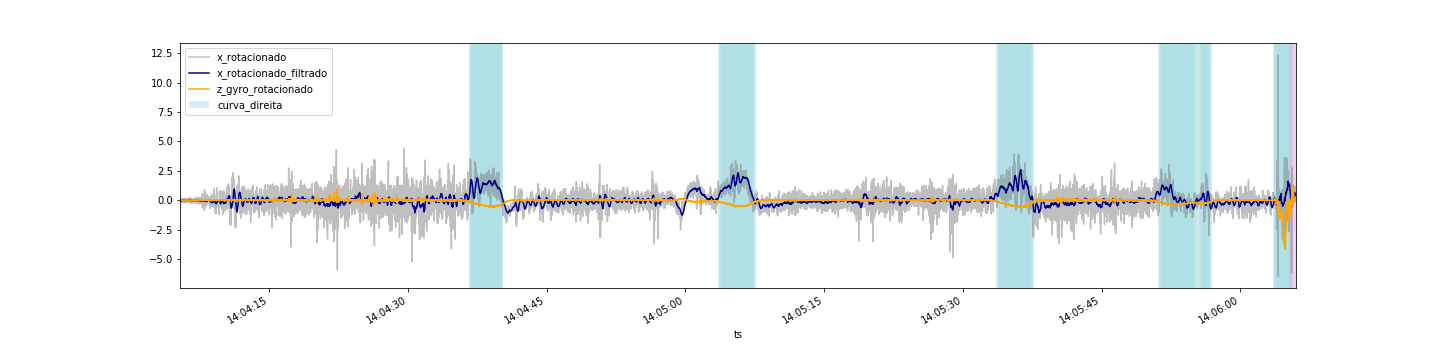
\includegraphics[height=70mm,width=\textwidth]{Figuras/eventosXGtrip2.png}}
    \caption{Assinatura de Eventos - Posição 2}
    \label{fig:eventosTrip2}
\end{figure}{}


\begin{figure}
    \centering
    \subfloat[Eventos no eixo $y$ do acelerômetro rotacionado.]{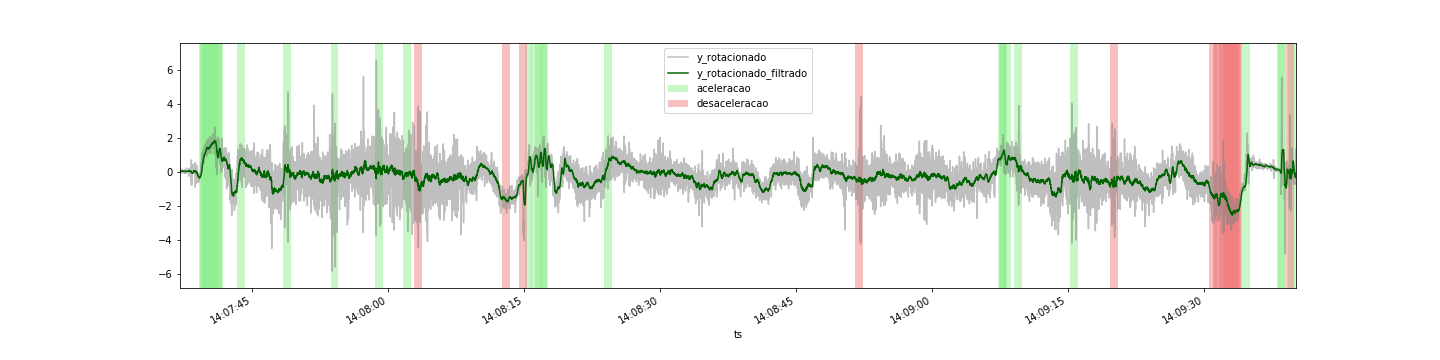
\includegraphics[height=70mm,width=\textwidth]{Figuras/eventosYtrip3.png}}
    \\
    \subfloat[Eventos no eixo $x$ do acelerômetro rotacionado e $z$ do giroscópio rotacionado.]{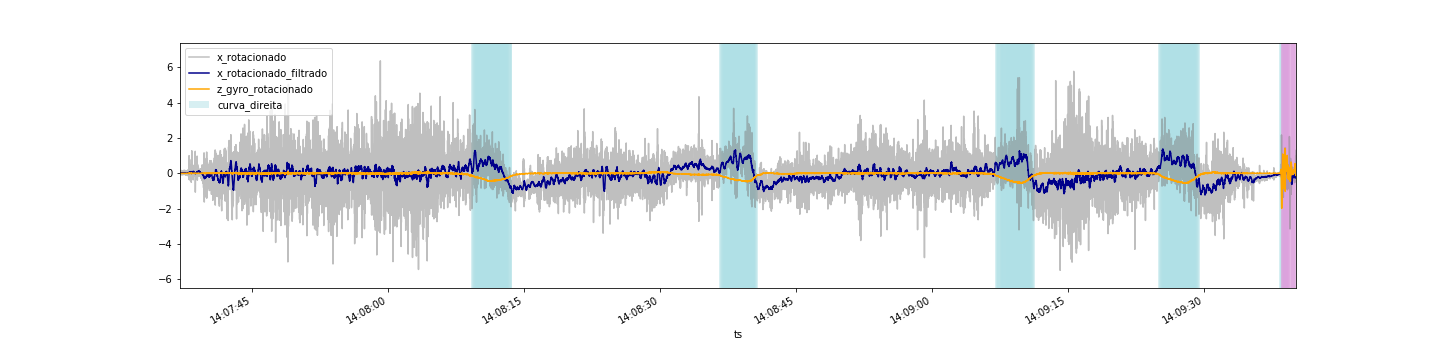
\includegraphics[height=70mm,width=\textwidth]{Figuras/eventosXGtrip3.png}}
    \caption{Assinatura de Eventos - Posição 3}
    \label{fig:eventosTrip3}
\end{figure}{}



\chapter{Conclusão}\label{Conclusão}




% ---


% ----------------------------------------------------------
% Anexos
% ----------------------------------------------------------

% ---
% Inicia os anexos
% ---

%---------------------------------------------------------------------
% INDICE REMISSIVO
%---------------------------------------------------------------------

\printindex

%---------------------------------------------------------------------
% Formulário de Identificação (opcional)
%---------------------------------------------------------------------

\end{document}
